%%%%%%%%%%%%%%%%%%%%%%%%%%%%%%%%%%%%%%%%%%%%%%%%%%%%%
%% File: main.tex
%% Author: John Liaperdos (ioannis.liaperdos@gmail.com)
%% Last update: April 28, 2015
%% Description: Provides an example of a PhD Thesis 
%% using the teipel-thesis-en pdfLaTeX class.
%%
%% Character encoding: UTF-8
%%%%%%%%%%%%%%%%%%%%%%%%%%%%%%%%%%%%%%%%%%%%%%%%%%%%%
%
%
%%%%%%
% 1. use the "modern" or "classic" option to switch between 
% a modern or classic font, respectively.
%
% 2. add/remove the "hyperref" option to enable/disable hyperlinks:
% (remember to remove auxiliary files after adding/removing 
% the "hyperref" option).
%
% 3. add/remove the "printer" option to typeset a printer-friendly 
% (grayscale)/color version of the thesis.
%
% 4. use the "watermark" option to indicate a draft copy of the thesis
%
% 5. use the "histinit" option to enable "historiated initials".
% (If used, all chapter initials declared by the \InitialCharacter{}
% macro are enlarged. If ommitted, arguments of \InitialCharacter{}
% are typeset as normal text.)
%
% 6. use the "plain" option to disable tikz graphics in title page
% and part/chapter headers (might help to avoid compilation timeouts).
% Note that "plain" disables CD label and CD cover creation.
%
% 7. use the "noindex" option to (hopefully) avoid compilation timeouts
% when compiling online (disables index generation - note that "\indexGR",
% "\index" invocations need not be removed when toggling this option).
%
% 8. use the "frontispiece" option to typeset a frontispiece at the back of the cover page
%
% 9. use the `letter' option for a US letter page layout, instead of A4
%
%%%%%%%%%%%%%%%%%%%%%%%%%%%%%%%%%%%%%%%%%%%%%%%%%%%%%%%%%%%%%%%%%%%%%%%%%%%%%%%
%
	  %\documentclass[modern,hyperref,watermark,histinit,frontispiece,plain]{teipel-thesis-en}
	   \documentclass[classic, hyperref,watermark,histinit,frontispiece,plain]{teipel-thesis-en} %%moder pone el formato lindo, pero los simbolos griegos no
%
\graphicspath{{figures/}}
%\usepackage[scientific-notation=true]{siunitx}
%\usepackage[spanish]{babel}
%\usepackage[spanish]{babel}
\usepackage{graphicx}%, color}
\graphicspath{{figures/}}
\usepackage{amsmath}
\usepackage{amscd}
\usepackage{feynmp}
\DeclareGraphicsRule{*}{mps}{*}{}
\usepackage{tikz-feynman}
\tikzfeynmanset{compat=1.1.0}
\usepackage{youngtab}
\usepackage{titlesec}
%\usepackage[latin1]{inputenc}
%\usepackage[utf8]{inputenc}
\usepackage{listings}
\usepackage{enumerate}
\usepackage{amssymb}
\usepackage{amsthm}
\usepackage{simplewick}
\usepackage{syntonly}
\usepackage{fancyhdr}
\usepackage{cancel}
\usepackage{siunitx}
\usepackage{slashed}
\usepackage{bbm}
\usepackage{dsfont}
%
\usepackage{multirow}
\usepackage{gensymb}
\usepackage{cite} % to collet the references
\usepackage{fancyhdr}
\pagestyle{fancy}
\fancyhf{}
\usepackage{dsfont}
\usepackage{float}

\usepackage{fancyhdr}
\pagestyle{fancy}
\fancyhf{}
\fancyhead[LO]{\leftmark} % En las p\'{a}ginas impares, parte izquierda del encabezado, aparecer\'{a} el nombre de cap\'{\i}tulo
\fancyhead[RE]{\rightmark} % En las p\'{a}ginas pares, parte derecha del encabezado, aparecer\'{a} el nombre de secci\'{o}n
\fancyfoot[C]{\thepage} % N\'{u}meros de p\'{a}gina en el centro

%%size
\setlength{\oddsidemargin}{-0.2 cm}
\setlength{\evensidemargin}{-0.2 cm}
\setlength{\textwidth}{16.2 cm}

%%%%%%%%%%%%%%%%%%%%%
%% UNIVERSITY INFO 
%%%%%%%%%%%%%%%%%%%%%%%%%%%%%%%%%%%%%%%%%%%%%%%%%%%%
%
% University Name
%
	\UniversityName{Universidad de Antioquia}
%
% School Name
%
	\SchoolName{Instituto de Física}
%
% Department Name
%
	\DepartmentName{Facultad de Ciencias Exactas y Naturales \\
						{\large{Grupo de fenomenología e interacciones fundamentales }} }
%
% Location
%
	\UniversityLocation{Medellín}
%
%
%%%%%%%%%%%%%%%%%%%%%%%%%%%%%%%%%%%%%%%%%%%%%%%%%%%%
%% THESIS INFO 
%%%%%%%%%%%%%%%%%%%%%%%%%%%%%%%%%%%%%%%%%%%%%%%%%%%%
%
%% -------------------------------------------------------------------
% Thesis Type
%
	\ThesisType{\\Pregrado}
%
%% -------------------------------------------------------------------
% Thesis Title 
%
% To force line breaks in title, use "\\".
% If different line break locations are to be used for the cover page and the inner title page (page 3) 
% repeat the cover page title as an optional argument of the \title macro, including line breaks.
%
% Examples:
% 1. Automatic title line breaks in cover page and inner title page: 
%	    \title{This is my title}
% 2. Title breaking after ''my'' in both cover page and inner title page:
%	    \title{This is my \\ title}
% 3. Title breaking after ''my'' in cover page, and after ''is'' in inner title page:
%	    \title[This is my \\ title]{This is \\ my title}
%
	\title{ Generación de asimetría bariónica a través de la leptogénesis 
  }
%%
%
%% -------------------------------------------------------------------
%% Thesis subtitle (optional)
%
% If no subtitle is required, set argument to blank, or comment-out the \subtitle macro.
%
% Example:
%%	\subtitle{This is my subtitle}
%%	\subtitle{with this subtitle}
%
%% -------------------------------------------------------------------
%
%% Author name
%
% For more than one authors, separate with ",".
% Example:
%	\authorName{Albert Einstein, George W. Bush} 
	\authorName{Katherine Builes Londoño} 
%
%% -------------------------------------------------------------------
%
%% Supervisor's name
% 
	\supervisor{Diego A. Restrepo Quintero }
	%\cosupervisor{Richard Feynman  }
%
%% -------------------------------------------------------------------
%% Supervisor's title
%
	\supervisorTitle{}
%
%
%% -------------------------------------------------------------------
%% Place and date of publication
%
	\thesisPlaceDate{Medellín, 2018}
%
%% -------------------------------------------------------------------
%% Place and date in acknowledgements (if applicable).
%
	\ackPlaceDate{Medellín, 2018}
%
%% -------------------------------------------------------------------
%% Approval information
%
	\examinationDate{ Date:}
	\approvalStatement{Approved by \hspace{2.0 cm}}
%
%% -------------------------------------------------------------------
%% Copyright Year
%
%	\copyrightYear{Creative Commons Wikipedia-like}
%
%% -------------------------------------------------------------------
%% Name of first examiner
%
%	\firstExaminer{Professor A}
	\firstExaminer{\hspace{5.0 cm}}
%
%% -------------------------------------------------------------------
%% Title of first examiner
%
	\firstExaminerTitle{}
%
%% -------------------------------------------------------------------
%% Name of second examiner
%
	\secondExaminer{\hspace{5.0 cm}}
%
%% -------------------------------------------------------------------
%% Title of second examiner
%
	\secondExaminerTitle{}
%%
%%
%%%%%%%%%%%%%%%%%%%%%%%%%%%%%%%%%%%%%%%%%%%%%%%%%%%%%%%%%%%%%%%%%%%%%%
%% THESIS COLORS: 
%%%%%%%%%%%%%%%%%%%%%%%%%%%%%%%%%%%%%%%%%%%%%%%%%%%%%%%%%%%%%%%%%%%%%%
%%
%% Color for cover and chapters
	\chaptercolor{brown!75!magenta}
%%
%% Color for appendices
	\appendixcolor{brown!80!magenta}
%%
%% hyperlink color (ignored if the "hyperref" option is omitted)
    	\hyperlinkcolor{red!55!brown}
%%
%% Thesis title foreground color in cover page (ignored if the "plain" option is used)
    	\titlecolor{white}
%%
%% Thesis title background color in cover page (ignored if the "plain" option is used)
    	\titlebackgroundcolor{brown!85!magenta}  
%%
%%
%%%%%%%%%%%%%%%%%%%%%%%%%%%%%%%%%%%%%%%%%%%%%%%%%%%%%%%%%%%%%%%%%%%%%%
%% COVER PAGE IMAGE: 
%%%%%%%%%%%%%%%%%%%%%%%%%%%%%%%%%%%%%%%%%%%%%%%%%%%%%%%%%%%%%%%%%%%%%%
%%
%% Cover page image (optional)
%% If no cover page image is required, set argument to blank, or comment-out the \coverpageimage macro.
%%
%% Syntax:
%%          \coverpageimage{scale factor}{path to cover page image}
%%      or
%%          \coverpageimage[tikz]{scale factor}{TikZ commands}
%%          (commands may include \usetikzlibrary statements, etc.)
%%      
%% Examples:
%%      - Use the image in "figures/rdf.png" scaled by 0.8 (=80%):
%%          \coverpageimage{0.8}{figures/rdf.png}
%%      - Use a TikZ drawing scaled by 0.5 (=50%):
%%          \coverpageimage[tikz]{0.5}{
%%              \draw[thick, magenta] \foreach \x in {18,90,...,306} {
%%                  (\x:4) node{} -- (\x+72:4)
%%                  (\x:4) -- (\x:3) node{}
%%                  (\x:3) -- (\x+15:2) node{}
%%                  (\x:3) -- (\x-15:2) node{}
%%                  (\x+15:2) -- (\x+144-15:2)
%%                  (\x-15:2) -- (\x+144+15:2)
%%              };
%%          }
%%
     %\coverpageimage{0.4}{figures/neutrino_mass_diagram}
     %\coverpageimage{0.3}{figures/bullet2}  
     \vspace{2.0 cm}
%%
%%
%%%%%%%%%%%%%%%%%%%%%%%%%%%%%%%%%%%%%%%%%%%%%%%%%%%%%%%%%%%%%%%%%%%%%%
%% MISCELLANEOUS SETTINGS: 
%%%%%%%%%%%%%%%%%%%%%%%%%%%%%%%%%%%%%%%%%%%%%%%%%%%%%%%%%%%%%%%%%%%%%%
%%
% Path to University Logo (all supported formats are allowed)
	%\UniversityLogoPath{logo/teikal_logo.eps}
	\UniversityLogoPath{figures/logo-udea}
%
% Path to University Logo (grayscale version to be used with the `printer' option)
	\UniversityBWLogoPath{figures/logo-udea.eps}
%
% Scalefactor for University logos (1 for 100%)
	\LogoScaleFactor{1.1}
% Draft Indication (watermark text to be used with the `watermark' option)
	\draftIndication{}%poner algo debajo de superviso en la primera hoja
%
% Frontispiece settings (ignored if the `frontispiece' option is omitted)
%	Syntax: \setFrontispiece[scale factor]{path to frontispiece image}{frontispiece image legend}
	\setFrontispiece[0.3]{figures/logo-udea}{Universidad de Antioquia} %figura detras de la primera página ---> GUITARRA
%
%%%%%%%%%%%%%%%%%%%%%%%%%%%%%%%%%%%%%%%%%%%%%%%%%%%%%%%%%%%%%%%%%%%%%%
%
% add custom hyphenation rules here
%\hyphenation{} 
%
%%%%
%
%
%%%%
\begin{document}

\maketitle
Generación de asimetría bariónica a través de la leptogénesis
\beginfrontmatter
	
% Abstract (content in `abstract.tex')
	\begin{abstract}

Nuestra existencia, es la prueba irrefutable de la prevalesencia de la materia sobre la anti-materia. Analizamos la generación de la asimetría bariónica a partir del decaimiento de los neutrinos derechos $N_{R}$, los cuales son introducidos mediante el modelos de see-saw. Se obtuvo una expresión general para la violación CP producida durante el decaimiento de $N_{R}$, $\epsilon$, y una cota superior para la misma. El establecimiento de una jerarquía en la masa de los neutrinos permitió establecer la dependencia del neutrino derecho mas ligero con $\epsilon$.

   \begin{keywords}
    	Bariogénesis, asimetría, neutrinos, leptogenesis, 
   \end{keywords}

\end{abstract}

% Dedication
	\thesisDedication{``Todos somos muy ignorantes. Lo que ocurre es que no todos ignoramos las mismas cosas''  Albert Einstein}
% Acknowledgements (content in `acknowledgements.tex')
	%%%%%%%%%%%%%%%%%%%%%%%%%%%%%%%%%%%%%%%%%%%%%%%%%%%%%%%%%%%%%%%%%%
%%
%% use the starred version of the "acknowledgements" environment
%% to omit signatures from this section, e.g.:
%% \begin{acknowledgements*} ... \end{acknowledgements*}
%% 
%%%%%%%%%%%%%%%%%%%%%%%%%%%%%%%%%%%%%%%%%%%%%%%%%%%%%%%%%%%%%%%%%
\begin{acknowledgements}
Quiero agradecer a todas las personas que a lo largo de mis años de pregrado me brindaron su apoyo.

En especial, le agradezco al profesor Diego Restrepo; su paciencia, amabilidad y apoyo durante estos años. 
Al profesor Luis Alfredo Muñoz, su asesoría durante el desarrollo de esta tesis. 

A mis padres, por ser mis mejores motivadores.
A mi familia y amigos, por hacer parte de mi proyecto de vida.
\end{acknowledgements}
% Table of Contents
	\tableofcontents
% List of Figures
	%\listoffigures
% List of Illustrations
	%\listofillustrations
% List of Tables
	%\listoftables
% Preface (content in `preface.tex') 
	%\begin{preface}
	Preface goes here ...  
\end{preface}
	
\beginmainmatter

%%%%%%%%%%%%%%%%%%%%%%%%%%%%%%%%%%%%%%%%%%%%%%%%%%%%%
%% INCLUDE YOUR CHAPTERS/SECTIONS HERE
%%
% Introduction
	\chapter{Introducción} 
%
\InitialCharacter{E}xplicar el origen del universo se ha convertido en una de las tareas más importantes de la comunidad científica, S. Hawking argumentaba: ``mi único objetivo es poder entender las razones por las cuales el universo es tal como es''~\cite{boslough1989stephen}. De los momentos iniciales del universo tenemos poca información, la teoría del Big Bang supone que todo comenzó con una gran explosión, según S. Hawking todo lo que ocurrió antes no tiene importancia~\cite{tyson_hawking_2018}. Una de las incógnitas que nos explica el Big Bang, es el porqué de la homogeneidad e isotropía del universo, La teoría de la inflación da explicación a estas incógnitas suponiendo que el universo sufrió una  expansión acelerada (exponencial)~\cite{Guth:1981}. Más tarde, A. Linde realiza correcciones a la idea inicial de Guth, la teoría está basada en un potencial asociado con un campo escalar (inflaton) a medida que el potencial sufre variaciones el universo se expande y por tanto, se enfría. Luego de las variaciones que sufre el potencial este comienza a oscilar alrededor de su mínimo, la energía producida en las oscilaciones se transforma en la energía necesaria para el surgimiento de materia y anti-materia~\cite{Linde:1981mu}. Se produce el decaimiento de partículas masivas, de igual forma, debido a las altas temperaturas que dominan el universo el proceso inverso también se produce. La expansión del universo trae como consecuencia una baja en la temperatura. A medida que la temperatura disminuye, se produce de forma sistemática, en función de la masa de las partículas, una imposibilidad de producir los procesos inversos. Se empieza a producir la aniquilación entre partículas y anti-partículas. Por lo cual, se esperaría que existiera una simetría entre ellas, es decir:%
% * <restrepo@udea.edu.co> 2018-05-29T14:30:58.359Z:
% 
% Aclarar que no es en un sólo paso
% 
% ^.
\begin{equation}
n_{B}=	n_{\overline{B}}\, ,
\end{equation}
%
La existencia de universo, planetas y habitantes, no es posible si esta simetría permanece exacta. Las observaciones muestran que en realidad~\cite{PDBook}
%
\begin{align}
\frac{n_{B}-n_{\overline{B}}}{n_{\gamma}}=10^{-10}\, .
\end{align}
%
Lo cual significa, que por cada $10^{10}+1$ barión existen $10^{10}$ anti-bariones. Por tanto, en algún momento se debió generar una asimetría entra bariónes y antibariónes. El proceso mediante el cual se genera esta asimetría, recibe el nombre bariogénesis.
En 1967 el físico ruso A. Sájarov estableció tres condiciones que debería cumplir una teoría que tratara de explicar la asimetría~\cite{Sakharov:1967dj}: la primera de ellas sostiene que Para producirse una asimetría bariónica  es necesario que en ciertas interacciones el número bariónico no se conserve 
%
% * <restrepo@udea.edu.co> 2018-05-29T14:36:31.541Z:
%
% ^.
%
La segunda se relaciona con el concepto de carga y paridad. El concepto de carga ($C$) está relacionado con el hecho de transformar partículas en anti-partículas. La paridad transforma un electrón derecho en un izquierdo. Para producirse un universo asimétrico era necesario una violación $CP$. La tercera es que se produzca una pérdida de equilibrio termodinámico, esto se sustenta con el hecho de que cuando existe equilibrio termodinámico y se produce una desintegración es totalmente factible que se produzca la desintegración inversa, manteniendo la simetría del universo.
Existen varios mecanismos que  cumplen con estas condiciones, el modelo de leptogénesis es uno de ellos. Este modelo fue propuesto por M.  Fukugita y T. Yanagida,  en 1986~\cite{Fukugita:1986hr}. La leptognesis se basa en la generación de asimetría, a partir, del decaimiento de neutrinos derechos, los cuales son introducidos a través del mecanismo see-saw. El mecanismo introduce tres nuevas partículas masivas, sus acoples e interacciones de Yukawa proveen las fuentes necesarias para producir la violación CP y el alejamiento del equilibrio térmico.
Nosotros centraremos nuestro zona de estudio en el momento en el cual existió el desequilibrio termodinámico que permitió a los neutrinos desacoplarse de las demás partículas forman un plasma. Por tal razón, implementamos el uso de doblete leptónico y escalar de Higgs.
%
\begin{align}
-\mathcal{L}=\lambda_{ij}^*\epsilon_{ab}   H^{\dagger b}{l^\dagger}^a_i {N_R}_j+\frac{1}{2}{M_R}_i {N_R}_i {N_R}_i+h.c \, ,
\end{align}
donde hemos definido
\begin{align}
  H=\begin{pmatrix}
H^{\dagger}\\
H^{0}
\end{pmatrix}\, & L=\begin{pmatrix}
\nu\\
e_{l}
\end{pmatrix}\, . 
\end{align}
%
Además, ${M_R}_i$ corresponde a las masas de Majorana de los neutrinos derechos. Después de producirse la ruptura de simetría, adquieren una masa de Dirac. 
% * <restrepo@udea.edu.co> 2018-05-29T14:44:40.038Z:
% 
% Comprobar notación para M_R
% 
% ^.
%
\begin{align}
-\mathcal{L}&=M^{i}_{D}\nu_{li}^{\dagger}N_{R}+\frac{1}{2}{M_R}_{i} {N_R}_i {N_R}_i\nonumber\\
&=\frac{1}{2}M^{i}_{D}\nu_{li}^{\dagger}N_{R}+\frac{1}{2}M^{i}_{D}\nu_{li}^{\dagger}N_{R}+\frac{1}{2}{M_R}_{i} {N_R}_i {N_R}_i\nonumber\\
&=\frac{1}{2} \begin{pmatrix} \nu_{l}^{\dagger}&N_{R}  \end{pmatrix} \begin{pmatrix}
0_{3x3}&M_{D}\\
M^{T}_{D}&M_{R}
\end{pmatrix}\begin{pmatrix} \nu_{l}^{\dagger}\\N_{R}  \end{pmatrix}
\end{align}
Definiendo 
$\chi=\begin{pmatrix} \nu_{l}^{\dagger}\\N_{R}  \end{pmatrix}$, y la matriz de masa 
$M_{\chi}=\begin{pmatrix}0_{3X3}&M_{D}\\M^{T}_{D}&M_{R}  \end{pmatrix}$
La matriz tiene los siguientes auto-valores
\begin{align}
M_{\chi_{\pm}}&=\frac{1}{2}\left[M_{R}\pm(M^{2}_{R}+4M_{D}M^{T}_{D})^{\frac{1}{2}}\right]\nonumber \\
&=\frac{1}{2}\left[M_{R}\pm M_{R}(1+{4M_{D}M^{-2}_{R}M^{T}_{D}})^{\frac{1}{2}}\right]
\end{align}
$M_{R}\gg M_{D}M^{T}_{D}$.
Por lo cual, se obtiene
\begin{align}
M_{\chi_{\pm}}=\frac{M_{R}}{2}[1\pm(2M_{D}M^{-2}_{R}M^{T}_{D})]\, .
\end{align}
Entonces
\begin{align}
M_{\chi_{-}}&=-M_{D}M^{-1}_{R}M^{T}_{D}\nonumber \\
M_{\chi_{+}}&=M_{R}\, .
\end{align}
La asimetría leptónica pasa a convertirse en asimetría bariónica, mediante un proceso mediado por esfalerones~\cite{Biswas:2017tce}. Estos procesos se caracterizan por la conservación de $B-L$ pero por la violación de $B+L$. Tanto $B$ como $L$ se escriben en términos $B-L$, de modo que, al generarse una asimetría leptónica se transfiere a una asimetría bariónica 
% Parts/Chapters
%	\part{Part A}
\chapter{Capitulo principal}
%
\InitialCharacter{E}n adicion a los dobletes del modelo estándar $l_i$ y $H$, nosotros introducimos campos de Weyl de derechos, ${N_R}_i$. El lagrangiano es 
%
\begin{align}
-\mathcal{L}=\lambda_{ij}\epsilon_{ab} \left( N_R \right)^\dagger_{j} l^a_iH^{b} +\lambda_{ij}^*\epsilon_{ab}   H^{\dagger b}{l^\dagger}^a_i {N_R}_j
+\frac{1}{2}M_i {N_R}_i {N_R}_i+\frac{1}{2}M_i \left( N_R\right)^\dagger_i 
\left( N_R\right)^\dagger_i\, .
\end{align}
%
Donde hemos asumido que los neutrinos derechos están en la base diagonal.

Tomando en cuenta que el número fermiónico debe ser conservado, nosotros asumimos $N_R$ como una partícula: un elemento del subgrupo de Lorentz $(0,1/2)$, y $\left( N_R \right)^{\dagger}$ la correspondiente anti-partícula.  Con esta convención, si nosotros comenzamos con el decaimiento de un fermión (anti-fermión) finalizaremos con el número correspondiente a fermiones (anti-fermión) en el estado final.
 
De esta forma, nosotros consideramos los procesos
\begin{align}
  N_R \to& l  H^\dagger &  \left( N_R \right)^{\dagger}\to& l^{\dagger} H\, . 
\end{align}

Nosotros usamos la convención:
\begin{align}
 l\to \xi_{\alpha}=&\sum_s\int \frac{\operatorname{d}^3p}{(2\pi)^3\sqrt{2E_{\mathbf{p}}}} \left[ x_{\alpha}\left(s,\mathbf{p}\right) a_s e^{-i p\cdot x}+y_{\alpha}\left(s,\mathbf{p}\right) b_s^{\dagger} e^{i p\cdot x}  \right]\nonumber\\
  l ^{\dagger}\to \xi_{\dot{\alpha}}^{\dagger}=&\sum_s\int \frac{\operatorname{d}^3p}{(2\pi)^3\sqrt{2E_{\mathbf{p}}}} \left[ y_{\dot{\alpha}}^{\dagger}\left(s,\mathbf{p}\right) b_s e^{-i p\cdot x}+x_{\dot{\alpha}}^{\dagger}\left(s,\mathbf{p}\right) a_s^{\dagger} e^{i p\cdot x}  \right]\nonumber\\
 \left( N_R \right)^{\dagger}\to \eta^{\alpha}=&\sum_s\int \frac{\operatorname{d}^3p}{(2\pi)^3\sqrt{2E_{\mathbf{p}}}} \left[ x^{\alpha}\left(s,\mathbf{p}\right) b_s e^{-i p\cdot x}+y^{\alpha}\left(s,\mathbf{p}\right) a_s^{\dagger} e^{i p\cdot x}  \right] \nonumber\\
  N_R\to \eta^{\dagger\dot{\alpha}}=&\sum_s\int \frac{\operatorname{d}^3p}{(2\pi)^3\sqrt{2E_{\mathbf{p}}}} \left[ y^{\dagger\dot{\alpha}}\left(s,\mathbf{p}\right) a_s e^{-i p\cdot x}+x^{\dagger\dot{\alpha}}\left(s,\mathbf{p}\right) b_s^{\dagger} e^{i p\cdot x}  \right]\, ,
\end{align}
y la solución a la ecuación de Klein-Gordon 
\begin{align}
\phi(x)=&\int\operatorname{d}^3p\frac{1}{\sqrt{2w_{p}(2\pi)^{3}}}(ae^{-ipx}+b^{\dagger}e^{ipx}) \nonumber\\
\phi^\dagger(x)=&\int\operatorname{d}^3p\frac{1}{\sqrt{2w_{p}(2\pi)^{3}}}(be^{-ipx}+a^{\dagger}e^{ipx}).
\end{align}
La asimetria CP corresponde a la siguiente expresión:
\begin{align}
\label{asimetria}
\epsilon=\frac{|M|^2-|\overline{M}|^2}{|M|^2+|\overline{M}|^2}
\end{align}
Donde $M$ corresponde a la amplitud de dispersión para procesos que involucran partículas y $\overline{M}$ para procesos que involucran anti-partículas. La matriz de dispersión tiene la siguiente forma:
\begin{align}
|M|^2=|M_{t}|^2+|M_{l}|^2+2|M_{t}||M_{l}|
\end{align}
Donde $|M_{t}|$ corresponde a la dispersión a nivel árbol y $|M_{l}|$ corresponde a la dispersión nivel loop.

 A fin de calcular la dispersión a nivel árbol, nosotros necesitamos calcular
\begin{align}
  S^{(1)}=&-i \lambda^*\int \operatorname{d}^4 x : H^{\dagger} \cdot  l^{\dagger} N_R  : \,
  -i \lambda\int \operatorname{d}^4 x :\left(N_R\right)^\dagger   H\cdot  l : \nonumber\\
       =&-i \lambda^*\int \operatorname{d}^4 x :\xi^{\dagger} \eta^{\dagger}  \phi^{\dagger} :
       -i \lambda\int \operatorname{d}^4 x :\eta\xi  \phi:\,.
\end{align}
En orden de evaluar
\begin{align}
\label{narbol}
  S_{fi}=&-i\lambda^*\,\langle 0,l(\boldsymbol{p'}) , H^\dagger(\boldsymbol{q}) | \xi_{-}^{\dagger}(x)   \phi_-^{\dagger}(x)\eta^{\dagger}_+(x) | 0,0, N_R(\boldsymbol{p})\rangle \nonumber\\
  &-i\lambda\,\langle 0,l^\dagger(\boldsymbol{p'}) , H(\boldsymbol{q})| \xi_{-}(x)   \phi_- (x)\eta_+(x) | 0,0, N_R^\dagger(\boldsymbol{p})\rangle\,.
\end{align}
\begin{figure}[H]
  \centering
   \begin{tikzpicture}
  \begin{feynman}   
    \vertex (a) {\(\eta^{\dagger\dot{\alpha}}\)};
    \vertex [right=of a] (b);
    \vertex [above right=of b] (f1) {\(\xi_{{\dot{\alpha}}}^{\dagger}\)};
    \vertex [below right=of b] (c);
  
    \diagram* {
      (a) -- [anti fermion] (b) -- [fermion] (f1),
      (b) -- [scalar,edge label'=\(H\)] (c),
    };  
  \end{feynman} 
    \end{tikzpicture}
   %
  \begin{tikzpicture}
    \def\leglength{1}
    \begin{feynman}
      \vertex (a) {\(\eta^{{\alpha}}\)} ;
    \vertex [right=of a] (b);
    \vertex [above right=of b] (f1) {\(\xi_{\alpha}\)};
    \vertex [below right=of b] (c);
  \diagram* {
      (a) -- [fermion] (b) -- [anti fermion] (f1),
      (b) -- [scalar,edge label'=\(H^\dagger\)] (c),
    }; 
  \end{feynman}   
  \end{tikzpicture}
  \caption{Diagramás de Feynman de los elementos de la matriz S Eq . (\ref{narbol}).}
\end{figure}
Los operadores escalera cumplen las siguientes propiedades:
\begin{align}
a_p^{\dagger}|n_p\rangle=\sqrt{n_p+1}|n_p+1\rangle ,   a_p|n_p\rangle=\sqrt{n_p}|n_p-1\rangle\,,
\end{align}
además, se define el estado de una partícula
\begin{align}
|H\rangle=&\frac{1}{\sqrt{V}}a_p^{\dagger}|0\rangle\nonumber\\
|H\rangle^\dagger=&\frac{1}{\sqrt{V}}b_p^{\dagger}|0\rangle .
\end{align}
Por tanto, es posible definir:
\begin{align}
\phi(x)_+|H(k)\rangle=\int\operatorname{d}^3p\frac{1}{\sqrt{2w_{p}(2\pi)^{3}}}a_pe^{-ipx}\frac{1}{\sqrt{V}}a_k^{\dagger}|0\rangle\\
\label{p2}
\phi(x)_+|H(k)\rangle=\int\operatorname{d}^3p\frac{1}{\sqrt{2w_{p}(2\pi)^{3}}}e^{-ipx}\frac{1}{\sqrt{V}}[a_p,a_k^{\dagger}]|0\rangle\\
\label{3}
\phi(x)_+|H(k)\rangle=\int\operatorname{d}^3p\frac{1}{\sqrt{2w_p}}e^{-ipx}\frac{1}{\sqrt{V}}\delta^{3}(p-k)|0\rangle\\
\label{4}
\phi(x)_+|H(k)\rangle=\frac{1}{\sqrt{2w_{p}{}}}e^{-ikx}\frac{1}{\sqrt{V}}|0\rangle\,.
\end{align}
De igual forma se obtiene:
\begin{align}
\phi(x)^{\dagger}_+|H^\dagger(k)\rangle=\int\operatorname{d}^3p\frac{1}{\sqrt{2w_{p}(2\pi)^{3}}}b_pe^{-ipx}\frac{1}{\sqrt{V}}a_k^{\dagger}|0\rangle\\
\phi(x)^{\dagger}_+|H^\dagger(k)\rangle=\int\operatorname{d}^3p\frac{1}{\sqrt{2w_{p}(2\pi)^{3}}}e^{-ipx}\frac{1}{\sqrt{V}}[b_p,b_k^{\dagger}]|0\rangle\\
\phi(x)^{\dagger}_+|H^\dagger(k)\rangle=\int\operatorname{d}^3p\frac{1}{\sqrt{2w_p}}e^{-ipx}\frac{1}{\sqrt{V}}\delta^{3}(p-k)|0\rangle\\
\phi(x)^{\dagger}_+|H^\dagger(k)\rangle=\frac{1}{\sqrt{2w_{p}{}}}e^{-ikx}\frac{1}{\sqrt{V}}|0\rangle\,.
\end{align}
Teniendo en cuenta los anteriores resultados e implementando las siguientes relaciones
\begin{align}
  \eta_+^{\dagger}(x)|N_R (\boldsymbol{p},s)\rangle=&\frac{1}{\sqrt{2 E_{p} V}}y^{\dagger}(s,\mathbf{p})e^{-i p\cdot x}|0\rangle,&\langle l(\boldsymbol{p},s)|\xi_-^{\dagger}(x)=&\langle 0|\frac{1}{\sqrt{2 E_p V}}x^{\dagger}(s,\mathbf{p})e^{i p\cdot x}\,,
\end{align}
\begin{align}
\eta_+(x)|N_R ^\dagger(\boldsymbol{p},s)\rangle=&\frac{1}{\sqrt{2 E_{p} V}}x(s,\mathbf{p})e^{-i p\cdot x}|0\rangle,&\langle l_+^\dagger(\boldsymbol{p},s|\xi_-(x)=\langle 0|\frac{1}{2E_p V}y(s,\mathbf{p})e^{i p\cdot x}\,,
\end{align}
se obtiene:
\begin{multline}
S_{fi}^{(1)}=-i\displaystyle\sum_{s,s'}\int \operatorname{d}^{4}x \lambda^* \frac{1}{\sqrt{2E_{p'} V}}x^{\dagger}(s,\mathbf{p'})e^{ip'\cdot x}\frac{1}{\sqrt{2w_{q}V}}e^{iq\cdot x}\frac{1}{\sqrt{2E_{p'}V}}y^{\dagger}(s,\mathbf{p})e^{-i p\cdot x}\\
-i\int \operatorname{d}^{4}x \lambda \frac{1}{\sqrt{2E_p V}}x(s,\mathbf{p})e^{-ip\cdot x}\frac{1}{\sqrt{2w_{q}V}}e^{iq\cdot x}\frac{1}{\sqrt{2E_{p'}V}}y(s,\mathbf{p'})e^{i p'\cdot x}\,.
\end{multline}
\begin{align}
S_{fi}^{(1)}=\frac{1}{\sqrt{2E_{p'}V}}\frac{1}{\sqrt{2w_{k}V}}\frac{1}{\sqrt{2E_p V}}(-i)\displaystyle\sum_{s,s'}(2\pi)^4\delta^4({p-(p'+q)})[\lambda^* x^{\dagger}(s,\mathbf{p'})y^{\dagger}(s,\mathbf{p})+\lambda x(s,\mathbf{p})y(s,\mathbf{p'})]\, .
\end{align}
Por tanto, la amplitud de dispersión a nivel árbol adquiere la siguiente forma:
\begin{align}
iM_{t}=(-i)\displaystyle\sum_{s}\lambda_{ji}^* x^{\dagger}(s,\mathbf{p-q})y^{\dagger}(s,\mathbf{p})\\ \nonumber
i\overline{M_{t}}=(-i)\displaystyle\sum_{s}\lambda_{ji} x(s,\mathbf{p})y(s,\mathbf{p-q})\, .
\end{align}
Ahora, nosotros nos concentramos en obtener la amplitud de de dispersión a nivel loop,
En la figura \ref{fig2} se muestra una contribución a la auto-energía donde el estado final son anti-partículas, en este decaimiento el número leptónico  se conserva
\begin{align}
(N_{R}^{\dagger}lH)_{x_{1}}
(H^{\dagger}l^{\dagger} N_{R})_{x_{2}}
(N_{R}^{\dagger}lH)_{x_{3}}
\end{align}
\begin{figure}[H]
\label{f}
\centering
\begin{tikzpicture}
  \begin{feynman}
    \vertex  (a) {\(\eta_{{i}}\)};
    \vertex [right=of a,dot, label=0:\(x_{1}\)] (b);
    \vertex [above right=of b] (f1);
    \vertex [below right=of b] (c);
    \vertex [above right=of c,dot, label=180:\(x_{2}\)] (f2);
    \vertex [right=of f2] (f0);
    \vertex[right=of f0,dot, label=0:\(x_{3}\)] (f3);
    \vertex [above right=of f3] (f4);
    \vertex [below right=of f3] (f5);
 
    \diagram* {
      (a)-- [fermion] (b) %-- [anti fermion,quarter left,edge label={\(\xi_{{{i}}}\)}] (f1),

      (c) -- [scalar, quarter left, edge label=\(\phi\)] (b),
      (f2) -- [scalar,quarter left,edge label=\(\phi^\dagger\)] (c),
     % (f1) -- [quarter left,edge label={\(\xi_{k}\)} ] (f2),
        (b) -- [anti fermion, half left,edge label={\(\xi_{m}\hspace{4em}\xi_{m}^{\dagger}\)} ] (f2),
       
       (f2) -- [with arrow=0.99,edge label={\(\eta^{\dagger}_{{k}}\)} ](f0),
       (f0) -- [edge label={\(\eta_{k}\)}] (f3),
       (f4) -- [fermion,edge label={\(\xi_{j}\)}] (f3),
       (f3) -- [scalar,edge label'=\(\phi\)] (f5),
    };
  \end{feynman} 
 \end{tikzpicture}
 \caption{Diagrama de Feymann que representa los términos de la ecuación (\ref{1})}
 \label{fig2}
\end{figure}
\begin{align}
\label{1}
S=(-i)^{3}\lambda_{jk}\lambda^*_{mk}\lambda_{mi}\int\operatorname{d}^{4}x_{1}\operatorname{d}^{4}x_{2}
\operatorname{d}^{4}x_{3} &\,\langle 0,l^\dagger(\boldsymbol{p'}) , H(\boldsymbol{q} )|
\bcontraction{|}{\xi}{(x_1)}{\xi}
\xi(x_{1})\xi^\dagger(x_{2})
\bcontraction{|}{\xi}{(x_1)}{\xi}
\phi(x_{1})\phi^\dagger(x_{2})
\bcontraction{|}{\eta^{{\alpha\dagger}}}{(x_2)}{\eta}
\eta^{{\alpha\dagger}}(x_{2})\eta^{{\alpha}} (x_{3})\nonumber\\
&\eta^{{\alpha}}(x_{1})\xi(x_{3})\phi(x_{3})  | 0,0, N_R^{\dagger}(\boldsymbol{p})\rangle\, .
\end{align}
\begin{align}
\eta_+(x_1)|N_R ^\dagger(\boldsymbol{p},s)\rangle=&\frac{1}{\sqrt{2 E_{p'} V}}x(s,\mathbf{p})e^{-i p\cdot x_{1}}|0\rangle,&\langle l_+^\dagger(\boldsymbol{q},s|\xi_-(x_{3})=\langle 0|\frac{1}{\sqrt{2E_p V}}y(s,\mathbf{q})e^{i q\cdot x_{3}}\, .
\end{align}
\begin{align}
S=(-i)^3\lambda_{jk}\lambda^*_{mk}\lambda_{mi}\frac{1}{\sqrt{2E_p V}}\frac{1}{\sqrt{2E_{p'} V}}\frac{1}{\sqrt{2w_k V}}\overleftarrow{iS}(x_{1}-x_{2})i\Delta(x_{2}-x_{1})\overrightarrow{iS}(x_{3}-x_{2})\nonumber \\ e^{i p'\cdot x_{3}}e^{i q\cdot x_{3}}e^{-i p\cdot x_{1}}x(s,\boldsymbol{p})y(s,\boldsymbol{p'})\, ,
\end{align}
\begin{align}
S=&(-i)^{3}\lambda_{jk}\lambda^*_{mk}\lambda_{mi}\frac{1}{\sqrt{2E_p V}}\frac{1}{\sqrt{2E_{p'} V}}\frac{1}{\sqrt{2w_k V}}\int\operatorname{d}^{4}x_{1}\operatorname{d}^{4}x_{2}
\operatorname{d}^{4}x_{3} \frac{dk}{(2\pi)^4}\frac{dq_{2}}{(2\pi)^4}\frac{dq_{3}}{(2\pi)^4}\overleftarrow{iS}(k)i\Delta(q_{2})\overrightarrow{iS}(q_{3})\nonumber\\ 
&e^{-ik\cdot (x_{1}-x_{2})}e^{-iq_{2}\cdot (x_{2}-x_{2})}e^{-iq_{3}\cdot  (x_{3}-x_{2})}e^{ip'\cdot x_{3}}e^{i q\cdot x_{3}}e^{-i p\cdot x_{1}}x(s,\boldsymbol{p})y(s,\boldsymbol{p'})\, .
\end{align}
\begin{align}
\int\operatorname{d}^{4}x_{1}e^{-ik\cdot (x_{1})}e^{-ip\cdot (x_{1})}e^{-iq_{2}\cdot (x_{1})}=(2\pi)^4\delta(p+k-q_{2})\\ 
\int\operatorname{d}^{4}x_{2}e^{ik\cdot (x_{2})}e^{-iq_{2}\cdot (x_{2})}e^{iq_{3}\cdot (x_{2})}=(2\pi)^4\delta(q_{2}-k-q_{3})\\
\int\operatorname{d}^{4}x_{3}e^{iq\cdot (x_{3})}e^{ip'\cdot (x_{3})}e^{-iq_{3}\cdot (x_{3})}=(2\pi)^4\delta(q_{3}-p'-q).
\end{align}
\begin{align}
S={(-i)^3}\lambda_{jk}\lambda^*_{mk}\lambda_{mi}\frac{1}{\sqrt{2E_p V}}\frac{1}{\sqrt{2E_{p'} V}}\frac{1}{\sqrt{2w_q}}\int \frac{dk}{(2\pi)^4}\frac{dq_{2}}{(2\pi)^4}\frac{dq_{3}}{(2\pi)^4}\overleftarrow{iS}(k)i\Delta(q_{2})\overrightarrow{iS}(q_{3})\nonumber\\(2\pi)^4\delta(p+k-q_{2})(2\pi)^4\delta(q_{2}-k-q_{3})(2\pi)^4\delta(q_{3}-p'-q)x(s,\boldsymbol{p})y(s,\boldsymbol{p'})\, ,
\end{align}
  \begin{align}
S={(-i)^3}\lambda_{jk}\lambda^*_{mk}\lambda_{mi}\frac{1}{\sqrt{2E_p V}}\frac{1}{\sqrt{2E_{p'} V}}\frac{1}{\sqrt{2w_q V}}\int \frac{dk}{(2\pi)^4}\overleftarrow{iS}(k)i\Delta(p+k)\overrightarrow{iS}(p)\nonumber\\(2\pi)^4\delta(p-(p'+q))
x(s,\boldsymbol{p})y(s,\boldsymbol{p'})\, ,
\end{align}
\begin{align}
S=(-i)^3\lambda_{jk}\lambda^*_{mk}\lambda_{mi}\frac{1}{\sqrt{2E_p V}}\frac{1}{\sqrt{2E_{p'} V}}\frac{1}{\sqrt{2w_qV}}\delta(p-(p'-q))\overrightarrow{iS}(p)\nonumber \\ \int \frac{dk}{(2\pi)^4}(2\pi)^4i\Delta(p+k)\overleftarrow{iS}(k)x(s,\boldsymbol{p})y(s,\boldsymbol{p'})\, .
\end{align}
Utilizando las reglas de propagadores de Feynman para fermiones de dos componentes~\cite{Dreiner:2008tw} nosotros obtuvimos:
\begin{align}
S={(-i)^3}\lambda_{jk}\lambda^*_{mk}\lambda_{mi}\frac{1}{\sqrt{2E_p V}}\frac{1}{\sqrt{2E_{p'} V}}\frac{1}{\sqrt{2w_q V}}\delta(p-(p'-k))\\
\frac{ip.\bar{\sigma}}{p^2-M_{k}^2}\int \frac{dk}{(2\pi)^4} (2\pi)^4\frac{i}{(p+k)^2}\frac{ik.\bar{\sigma}}{k^2}x(s,\boldsymbol{p})y(s,\boldsymbol{p'})\, .
\end{align}
Por consiguiente, encontramos que la amplitud 
\begin{align}
i\overline{M_{l}}={(-i)^3}\lambda_{jk}\lambda^*_{mk}\lambda_{mi}
\frac{ip.\bar{\sigma}}{p^2-M_{k}^2}\int \frac{dk}{(2\pi)^4}\frac{i}{(p+k)^2}\frac{ik.\bar{\sigma}}{k^2}x(s,\boldsymbol{p})y(s,\boldsymbol{p-q}).
\end{align}
Para obtener un resultado más condensado nosotros usamos la función de Passarino~\cite{romao:2006}:
\begin{align}
\label{p1}
B^{\mu}=\frac{(2\pi\mu)^{4-d}}{i\pi^2}\int d^{d}k^4k^{\mu}\prod_{i=0}^{1}\frac{1}{(k+r_{i})^2-m_{i}^2}\,,
\end{align}
estableciendo $r_{0}=0$ $r_{1}=p$
\begin{align}
\label{p2}
B^{\mu}=\frac{(2\pi\mu)^{4-d}}{i\pi^2}\int d^{d}k^{\mu}\frac{1}{k-m_{0}^2}\frac{1}{(k+p)^2-m_{1}^2}\,,
\end{align}
utilizando $m_{0}=0$ $m_{1}=0$
\begin{align}
\label{p3}
B^{\mu}=\frac{(2\pi\mu)^{4-d}}{i\pi^2}\int dk^{d}\frac{k^{\mu}}{k^2}\frac{1}{(k+p)^2}\,.
\end{align}
Luego, nosotros obtuvimos
\begin{align}
i\overline{M_{l}}={(-i)^3}\lambda_{jk}\lambda^*_{mk}\lambda_{mi}
\frac{ip.\bar{\sigma}}{p^2-M_{k}^2}\frac{i^3\pi^2B^\mu}{(2\pi)^4}{\overline{\sigma}}_{\mu} x(s,\boldsymbol{p})y(s,\boldsymbol{p-q}).
\end{align}
Utilizando la expresión de la integral en términos de funciones se obtiene~\cite{romao:2006}
\begin{align}
\label{p4}
B^{\mu}=r_{1}^{\mu}B_{1}(p^2,m_{0},m_{1}^2)
\end{align}
\begin{align}
i\overline{M_{l}}={(-i)^3}\lambda_{jk}\lambda^*_{mk}\lambda_{mi}
\frac{ip.\bar{\sigma}}{p^2-M_{k}^2}\frac{i^3\pi^2p^{\mu}B_{1}(p^2,0,0^2)}{(2\pi)^4}{\overline{\sigma}}_{\mu} x(s,\boldsymbol{p})y(s,\boldsymbol{p-q}),
\end{align}

\begin{align}
i\overline{M_{l}}=i\lambda_{jk}\lambda^*_{mk}\lambda_{mi}
\frac{p^2}{p^2-M_{k}^2}\frac{B_{1}(p^2,0,0)}{16\pi^2} x(s,\boldsymbol{p})y(s,\boldsymbol{p-q})\, . 
\end{align}
Debido a que estamos considerando Neutrinos másivos, nosotros relacionamos $p^2=M_i$
\begin{align}
i\overline{M_{l}}=i\lambda_{jk}\lambda^*_{mk}\lambda_{mi}
\frac{M_{i}}{M_{i}-M_{k}^2}\frac{B_{1}(p^2,0,0)}{16\pi^2} x(s,\boldsymbol{p})y(s,\boldsymbol{p-q})\, . 
\end{align}
En la figura \ref{fig3} el estado final son anti-partículas. A diferencia de la situación anterior; en esta no se conservar el número leptónico  
\begin{align}
(H^{\dagger}l^{\dagger}N_{R})_{X_{1}}
(N_{R}^{\dagger}lH)_{x_{2}}
(N_{R}^{\dagger}lH)_{x_{3}}
\end{align}
\begin{figure}[H]
\centering
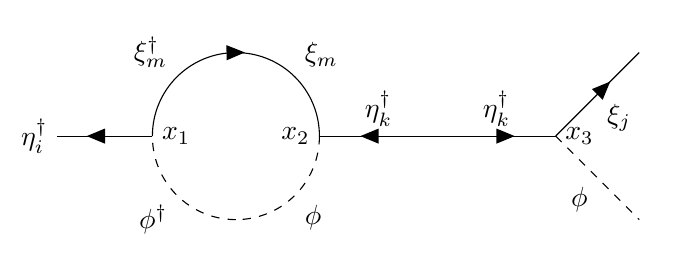
\begin{tikzpicture}
  \begin{feynman}
    \vertex  (a) {\(\eta^{\dagger}_{{i}}\)};
    \vertex [right=of a,dot, label=0:\(x_{1}\)] (b);
    \vertex [above right=of b] (f1);
    \vertex [below right=of b] (c);
    \vertex [above right=of c,dot, label=180:\(x_{2}\)] (f2);
    \vertex [right=of f2] (f0);
    \vertex[right=of f0,dot, label=0:\(x_{3}\)] (f3);
    \vertex [above right=of f3] (f4);
    \vertex [below right=of f3] (f5);
 
    \diagram* {
      (a)-- [anti fermion] (b) -- [with arrow=0.99,quarter left,edge label={\(\xi^{\dagger} _{{{m}}}\)}] (f1),

      (c) -- [scalar, quarter left, edge label=\(\phi^{\dagger}\)] (b),
      (f2) -- [scalar,quarter left,edge label=\(\phi\)] (c),
      (f1) -- [quarter left,edge label={\(\xi_{m}\)} ] (f2),
       
       (f2) -- [anti fermion,edge label={\(\eta^{\dagger}_{{k}}\)} ](f0),
       (f3) -- [anti fermion, edge label'={\(\eta^{\dagger}_{k}\)}] (f0),
       (f4) -- [anti fermion,edge label={\(\xi_{j}\)}] (f3),
       (f3) -- [scalar,edge label'=\(\phi\)] (f5),
    };
  \end{feynman} 
 \end{tikzpicture}
 \caption{Diagrama de Feymann que representa los términos de la ecuación (\ref{2})}
\label{fig3}
\end{figure}



\begin{align}
\label{2}
S={(-i)^{3}}\lambda_{jk}\lambda_{mk}\lambda^*_{mi}\int\operatorname{d}^{4}x_{1}\operatorname{d}^{4}x_{2}
\operatorname{d}^{4}x_{3} &\,\langle 0,l^\dagger(\boldsymbol{p'}) , H(\boldsymbol{q} )|
\bcontraction{|}{\xi}{(x_1)}{\xi}
\xi^\dagger(x_{1})\xi(x_{2})
\bcontraction{|}{\xi}{(x_1)}{\xi}
\phi^\dagger(x_{1})\phi(x_{2})
\bcontraction{|}{\eta^{{\alpha\dagger}}}{(x_2)}{\eta}
\eta^{{\alpha\dagger}}(x_{2})\eta^{{\alpha\dagger}} (x_{3})\nonumber\\
&\xi(x_{3})\phi(x_{3}) \eta^{\dagger{{\alpha}}}(x_{1}) | 0,0, N_R(\boldsymbol{p})\rangle.
\end{align}

\begin{align}
  \eta{(x)}^{\dagger}|N_R(\boldsymbol{p},s)\rangle=&\frac{1}{\sqrt{2 E_{p} V}}y^\dagger(s,\mathbf{p})e^{-i p\cdot x}|0\rangle,&\langle l(\boldsymbol{p},s)|\xi_-^{\dagger}(x)=&\langle 0|\frac{1}{\sqrt{2 E_p V}}y(s,\mathbf{p})e^{i p\cdot x}|0\rangle.
\end{align}

\begin{align}
S={(-i)^{3}}\lambda_{jk}\lambda_{mk}\lambda^*_{mi}\frac{1}{\sqrt{2E_p V}}\frac{1}{\sqrt{2E_{p'} V}}\frac{1}{\sqrt{2w_k V}}y(s,\boldsymbol{p'})\overrightarrow{iS}(x_{1}-x_{2})i\Delta(x_{2}-x_{1})\overrightarrow{\overleftarrow{iS}}(x_{3}-x_{2})\nonumber \\ e^{i p'\cdot x_{3}}e^{i k\cdot x_{3}}e^{-i p\cdot x_{1}}y^{\dagger}(s,\boldsymbol{p}),
\end{align}

\begin{align}
S=\frac{(-i)^{3}}{3}\lambda_{jk}\lambda^*_{mk}\lambda^*_{mi}\frac{1}{\sqrt{2E_p V}}\frac{1}{\sqrt{2E_{p'} V}}\frac{1}{\sqrt{2w_k V}}\int y(s,\boldsymbol{p'})\operatorname{d}^{4}x_{1}\operatorname{d}^{4}x_{2}
\operatorname{d}^{4}x_{3} \frac{dk}{(2\pi)^4}\frac{dq_{2}}{(2\pi)^4}\frac{dq_{3}}{(2\pi)^4}\overrightarrow{iS}(k)i\Delta(q_{2})\overrightarrow{\overleftarrow{iS}}(q_{3})\nonumber\\ 
e^{-iq_{1}\cdot (x_{1}-x_{2})}e^{-iq_{2}\cdot (x_{2}-x_{1})}e^{-iq_{3}\cdot (x_{3}-x_{2})}e^{i p'\cdot x_{3}}e^{i k\cdot x_{3}}e^{-i p\cdot x_{1}}y^{\dagger}(s,\boldsymbol{p}),
\end{align}

\begin{align}
S={(-i)^{3}}\lambda_{jk}\lambda^*_{mk}\lambda^*_{mi}\frac{1}{\sqrt{2E_p V}}\frac{1}{\sqrt{2E_{p'} V}}\frac{1}{\sqrt{2w_k V}}\int y(s,\boldsymbol{p'}) \frac{dk}{(2\pi)^4}\frac{dq_{2}}{(2\pi)^4}\frac{dq_{3}}{(2\pi)^4}\overrightarrow{iS}(q_{1})i\Delta(q_{2})\overrightarrow{\overleftarrow{iS}}(q_{3})\nonumber\\(2\pi)^4\delta(p+q_{1}-q_{2})(2\pi)^4\delta(q_{2}-k-q_{3})(2\pi)^4\delta(q_{3}-p'-q)y^{\dagger}(s,\boldsymbol{p}),
\end{align}

\begin{align}
S={(-i)^{3}}\lambda_{jk}\lambda^*_{mk}\lambda^*_{mi}\frac{1}{\sqrt{2E_p V}}\frac{1}{\sqrt{2E_{p'} V}}\frac{1}{\sqrt{2w_k V}}\delta(p-(p'+k))\overrightarrow{\overleftarrow{iS}}(p)\nonumber \\ \int \frac{dk}{(2\pi)^4}(2\pi)^4i\Delta(p+k){\overrightarrow{iS}}(k)y(s,\boldsymbol{p'})y^{\dagger}(s,\boldsymbol{p}).
\end{align}
\begin{align}
S={(-i)^{3}}\lambda_{jk}\lambda^*_{mk}\lambda^*_{mi}\frac{1}{\sqrt{2E_p V}}\frac{1}{\sqrt{2E_{p'} V}}\frac{1}{\sqrt{2w_k V}}\delta(p-(p'+k))\\
\frac{iM_{k}}{p^2-M_{k}^2}\int y(s,\boldsymbol{p'}) \frac{dk}{(2\pi)^4}(2\pi)^4\frac{i}{(p+k)^2}\frac{ik.{\sigma}}{k^2}y^{\dagger}(s,\boldsymbol{p})\, . 
\end{align}
Luego 
\begin{align}
i\overline{M_{l}}={(-i)^{3}}\lambda_{jk}\lambda^*_{mk}\lambda^*_{mi}\frac{iM_{k}}{p^2-M_{k}^2}\int \frac{dk}{(2\pi)^4}\frac{i}{(p+k)^2}\frac{ik.{\sigma}}{k^2}y(s,\boldsymbol{p'})y^{\dagger}(s,\boldsymbol{p})\, . 
\end{align}
Usando las ideas desarrolladas entre las Eq.(\ref{p1})-(\ref{p3})y (\ref{p4}) nosotros obtuvimos 
\begin{align}
i\overline{M_{l}}=\frac{{(-i)^{3}}}{16\pi^4}\lambda_{jk}\lambda^*_{mk}\lambda^*_{mi}\frac{iM_{k}}{p^2-M_{k}^2}(i)^3\pi^2y(s,\boldsymbol{p'})p^{\mu}B_{1}(p^2,0,0){\sigma}_{\mu}y^{\dagger}(s,\boldsymbol{p})\, . 
\end{align}
Utilizando las ecuaciones de momentum de Dirac~\cite{Dreiner:2008tw}
\begin{align}
i\overline{M_{l}}=\frac{i}{16\pi^2}\lambda^*_{jk}\lambda^*_{mk}\lambda^*_{mi}\frac{M_{k}M_{i}}{M_i^2-M_{k}^2}B_{1}(p^2,0,0)y(s,\boldsymbol{p-q})x(s,\boldsymbol{p})\, . 
\end{align}
En la figura \ref{fig4} se muestra una contribución a la auto-energía donde el estado final son partículas, en este decaimiento el número leptónico  se conserva.
\begin{align}
(H^{\dagger}l^{\dagger} N_{R})_{x_{1}}
(N_{R}^{\dagger}lH)_{x_{2}}
(H^{\dagger}l^{\dagger} N_{R})_{x_{3}}
\end{align}

\begin{figure}[H]
\centering
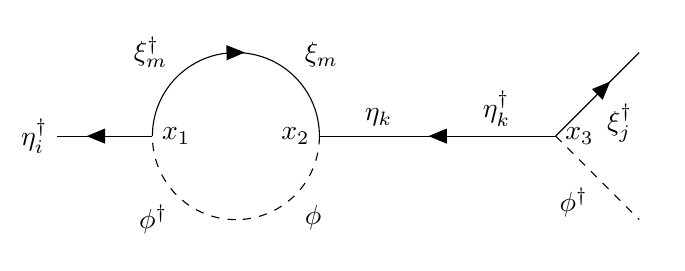
\begin{tikzpicture}
  \begin{feynman}
    \vertex  (a) {\(\eta^{\dagger}_{{i}}\)};
    \vertex [right=of a,dot, label=0:\(x_{1}\)] (b);
    \vertex [above right=of b] (f1);
    \vertex [below right=of b] (c);
    \vertex [above right=of c,dot, label=180:\(x_{2}\)] (f2);
    \vertex [right=of f2] (f0);
    \vertex[right=of f0,dot, label=0:\(x_{3}\)] (f3);
    \vertex [above right=of f3] (f4);
    \vertex [below right=of f3] (f5);
    \diagram* {
      (a)-- [anti fermion] (b) -- [with arrow=0.99,quarter left,edge label={\(\xi^{\dagger}_{{{m}}}\)}] (f1),

      (c) -- [scalar, quarter left, edge label=\(\phi^{\dagger}\)] (b),
      (f2) -- [scalar,quarter left,edge label=\(\phi\)] (c),
      (f1) -- [quarter left,edge label={\(\xi_{m}\)} ] (f2),
       
       (f2) -- [edge label={\(\eta_{{k}}\)} ](f0),
       (f3) -- [with arrow=0.99, edge label'={\(\eta^{\dagger}_{k}\)}] (f0),
       (f4) -- [anti fermion,edge label={\(\xi^{\dagger}_{j}\)}] (f3),
       (f3) -- [scalar,edge label'=\(\phi^{\dagger}\)] (f5),
    };
  \end{feynman} 
 \end{tikzpicture}
 \caption{Diagrama de Feymann que representa los términos de la ecuación (\ref{4})}
 \label{fig4}
\end{figure}
\begin{align}
\label{4}
S=(-i)^3\lambda^ *_{jk}\lambda_{mk}\lambda^*_{mi}\int\operatorname{d}^{4}x_{1}\operatorname{d}^{4}x_{2}
\operatorname{d}^{4}x_{3} &\,\langle 0,l(\boldsymbol{p'}) , H^{\dagger}(\boldsymbol{q} )|
\bcontraction{|}{\xi}{(x_1)}{\xi}
\xi^{\dagger}(x_{1})\xi(x_{2})
\bcontraction{|}{\phi}{(x_1)}{\phi}
\phi^{\dagger}(x_{1})\phi(x_{2})
\bcontraction{|}{\eta^{{\alpha}}}{(x_2)}{\eta}
\eta^{{\alpha}}(x_{2})\eta^{{\alpha\dagger}}(x_{3})\nonumber\\
&\eta^{\alpha\dagger}(x_{1})\xi^{\dagger}(x_{3})\phi^{\dagger}(x_{3})  | 0,0, N_R(\boldsymbol{p})\rangle.
\end{align}
\begin{align}
  \eta_+^{\dagger}(x)|N_R (\boldsymbol{p},s)\rangle=&\frac{1}{\sqrt{2 E_{p} V}}y^{\dagger}(s,\mathbf{p})e^{-i p\cdot x}|0\rangle,&\langle l(\boldsymbol{p},s)|\xi_-^{\dagger}(x)=&\langle 0|\frac{1}{\sqrt{2 E_p V}}x^{\dagger}(s,\mathbf{p})e^{i p\cdot x}\,,
\end{align}
\begin{align}
S=(-i)^{3}\lambda^ *_{jk}\lambda_{mk}\lambda^*_{mi}\overrightarrow{iS}(x_{1}-x_{2})i\Delta(x_{1}-x_{2})\overleftarrow{iS}(x_{2}-x_{3})\frac{1}{\sqrt{2E_p V}}\frac{1}{\sqrt{2E_{p'} V}}\frac{1}{\sqrt{2w_k V}}\nonumber\\ 
e^{i p'\cdot x_{3}}e^{i q\cdot x_{3}}e^{-i p\cdot x_{1}}x^\dagger(s,\boldsymbol{p'})y^\dagger(s,\boldsymbol{p}),
\end{align}
\begin{align}
S=(-i)^{3}\lambda^ *_{jk}\lambda_{mk}\lambda^*_{mi}\frac{1}{\sqrt{2E_p V}}\frac{1}{\sqrt{2E_{p'} V}}\frac{1}{\sqrt{2w_k V}}\int\operatorname{d}^{4}x_{1}\operatorname{d}^{4}x_{2}
\operatorname{d}^{4}x_{3} \frac{dk}{(2\pi)^4}\frac{dq_{2}}{(2\pi)^4}\frac{dq_{3}}{(2\pi)^4}\overrightarrow{iS}(q_{1})i\Delta(q_{2})\overleftarrow{iS}(q_{3})\nonumber\\ 
e^{-iq_{1}\cdot (x_{1}-x_{2})}e^{-iq_{2}\cdot (x_{2}-x_{1})}e^{-iq_{3}\cdot (x_{3}-x_{2})}e^{i p'\cdot x_{3}}e^{i q\cdot x_{3}}e^{-i p\cdot x_{1}}x^\dagger(s,\boldsymbol{p'})y^\dagger(s,\boldsymbol{p}),
\end{align}
\begin{align}
S=(-i)^{3}\lambda^ *_{jk}\lambda_{mk}\lambda^*_{mi}\frac{1}{\sqrt{2E_p V}}\frac{1}{\sqrt{2E_{p'} V}}\frac{1}{\sqrt{2w_q V}}\int \frac{dk}{(2\pi)^4}\frac{dq_{2}}{(2\pi)^4}\frac{dq_{3}}{(2\pi)^4}\overrightarrow{iS}(q_{1})i\Delta(q_{2})\overleftarrow{iS}(q_{3})\nonumber\\(2\pi)^4\delta(p+k-q_{2})(2\pi)^4\delta(q_{2}-k-q_{3})(2\pi)^4\delta(q_{3}-p'-q)x^\dagger(s,\boldsymbol{p'})y^\dagger(s,\boldsymbol{p}),
\end{align}
\begin{align}
S=(-i)^{3}\lambda^ *_{jk}\lambda_{mk}\lambda^*_{mi}\frac{1}{\sqrt{2E_p V}}\frac{1}{\sqrt{2E_{p'} V}}\frac{1}{\sqrt{2w_k V}}\delta(p-(p'+k))\overleftarrow{iS}(p)\nonumber \\ \int \frac{dk}{(2\pi)^4} (2\pi)^4 i\Delta(p+k)\overrightarrow{iS}(k)x^\dagger(s,\boldsymbol{p'})y^\dagger(s,\boldsymbol{p}),
\end{align}
\begin{align}
S=(-i)^{3}\lambda^ *_{jk}\lambda_{mk}\lambda^*_{mi}\frac{1}{\sqrt{2E_p V}}\frac{1}{\sqrt{2E_{p'} V}}\frac{1}{\sqrt{2w_k V}}\delta(p-(p'+k))\\
\frac{ip.\sigma}{p^2-M_{k}^2}\int \frac{dk}{(2\pi)^4}(2\pi)^4\frac{i}{(p+k)^2}\frac{ik.\bar{\sigma}}{k^2}x^\dagger(s,\boldsymbol{p'})y^\dagger(s,\boldsymbol{p})\, . 
\end{align}
Luego, nosotros obtuvimos
\begin{align}
iM_{l}=(-i)^{3}\lambda^ *_{jk}\lambda_{mk}\lambda^*_{mi}\frac{ip.\bar{\sigma}}{p^2-M_{k}^2}\int \frac{dk}{(2\pi)^4}\frac{i}{(p+k)^2}\frac{ik.\bar{\sigma}}{k^2}x^\dagger(s,\boldsymbol{p-q})y^\dagger(s,\boldsymbol{p})\, . 
\end{align}
Usando las ideas desarrolladas entre las Eq.(\ref{p1})-(\ref{p3})y (\ref{p4}) nosotros obtuvimos 
\begin{align}
iM_{l}=\frac{i}{16\pi^2}\lambda^*_{jk}\lambda_{mk}\lambda^*_{mi}
\frac{M_i^2}{M_i^2-M_{k}^2}B_{1}(p^2,0,0)x^\dagger(s,\boldsymbol{p-q})y^\dagger(s,\boldsymbol{p})\, . 
\end{align}
En la figura \ref{fig4} se muestra una contribución a la auto-energía donde el estado final son partículas, en este decaimiento el número leptónico  no se conserva.
\begin{align}
(N_{R}^{\dagger}lH)_{X_{1}}
(H^{\dagger}l^{\dagger}N_{R})_{X_{2}}
(H^{\dagger}l^{\dagger} N_{R})_{X_{3}}
\end{align}

\begin{figure}[H]
\label{fig5}
\centering
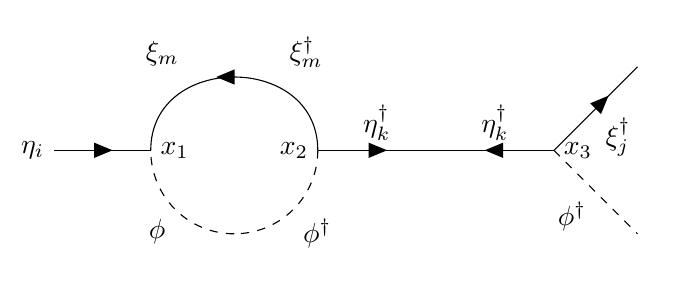
\begin{tikzpicture}
  \begin{feynman}
    \vertex  (a) {\(\eta_{{i}}\)};
    \vertex [right=of a,dot, label=0:\(x_{1}\)] (b);
    \vertex [above right=of b] (f1);
    \vertex [below right=of b] (c);
    \vertex [above right=of c,dot, label=180:\(x_{2}\)] (f2);
    \vertex [right=of f2] (f0);
    \vertex[right=of f0,dot, label=0:\(x_{3}\)] (f3);
    \vertex [above right=of f3] (f4);
    \vertex [below right=of f3] (f5);
 
    \diagram* {
      (a)-- [fermion] (b),

      (c) -- [scalar, quarter left, edge label=\(\phi\)] (b),
      (f2) -- [scalar,quarter left,edge label=\(\phi^{\dagger}\)] (c),
%(f1) -- [anti fermion,quarter left,edge label={\(\xi^{\dagger}_{m}\)} ] (f2),
       (b) -- [anti fermion, half left,edge label={\(\xi_{m}\hspace{4em}\xi_{m}^{\dagger}\)} ] (f2),
       (f2) -- [fermion,edge label={\(\eta^{\dagger}_{{k}}\)} ](f0),
       (f3) -- [fermion, edge label'={\(\eta^{\dagger}_{k}\)}] (f0),
       (f4) -- [anti fermion,edge label={\(\xi^{\dagger}_{j}\)}] (f3),
       (f3) -- [scalar,edge label'=\(\phi^{\dagger}\)] (f5),
    };
  \end{feynman} 
 \end{tikzpicture}
 \caption{Diagrama de Feymann que representa los términos de la ecuación (\ref{78})}
\end{figure}



\begin{align}
\label{78}
S=(-i)^{3}\lambda^*_{jk}\lambda^*_{mk}\lambda_{mi}\int\operatorname{d}^{4}x_{1}\operatorname{d}^{4}x_{2}
\operatorname{d}^{4}x_{3} &\,\langle 0,l(\boldsymbol{p'}) , H^\dagger(\boldsymbol{q} )|
\bcontraction{|}{\xi}{(x_1)}{\xi}
\xi(x_{1})\xi^\dagger(x_{2})
\bcontraction{|}{\xi}{(x_1)}{\xi}
\phi(x_{1})\phi^\dagger(x_{2})
\bcontraction{|}{\eta^{{\alpha\dagger}}}{(x_2)}{\eta}
\eta^{{\alpha\dagger}}(x_{2})\eta^{{\alpha\dagger}} (x_{3})\nonumber\\
&\xi^{\dagger}(x_{3})\phi^{\dagger}(x_{3}) \eta^{{\alpha}}(x_{1}) | 0,0, N_R^{\dagger}(\boldsymbol{p})\rangle\, ,
\end{align}

\begin{align}
  \eta_(x)|N_R^{\dagger} (\boldsymbol{p},s)\rangle=&\frac{1}{\sqrt{2 E_{p} V}}x(s,\mathbf{p})e^{-i p\cdot x}|0\rangle,&\langle l(\boldsymbol{p},s)|\xi_-^{\dagger}(x)=&\langle 0|\frac{1}{\sqrt{2 E_p V}}x^{\dagger}(s,\mathbf{p})e^{i p\cdot x}|0\rangle\, .
\end{align}

\begin{align}
S={(-i)^{3}}\lambda^*_{jk}\lambda^*_{mk}\lambda_{mi}\frac{1}{\sqrt{2E_p V}}\frac{1}{\sqrt{2E_{p'} V}}\frac{1}{\sqrt{2w_k V}}\overleftarrow{iS}(x_{1}-x_{2})i\Delta(x_{2}-x_{1})\overrightarrow{\overleftarrow{iS}}(x_{3}-x_{2})\nonumber \\ e^{i p'\cdot x_{3}}e^{i k\cdot x_{3}}e^{-i p\cdot x_{1}}x^{\dagger}(s,\boldsymbol{p'})x(s,\boldsymbol{p})\, ,
\end{align}

\begin{align}
S=\frac{(-i)^{3}}{3}\lambda^*_{jk}\lambda^*_{mk}\lambda_{mi}\frac{1}{\sqrt{2E_p V}}\frac{1}{\sqrt{2E_{p'} V}}\frac{1}{\sqrt{2w_k V}}\int\operatorname{d}^{4}x_{1}\operatorname{d}^{4}x_{2}
\operatorname{d}^{4}x_{3} \frac{dk}{(2\pi)^4}\frac{dq_{2}}{(2\pi)^4}\frac{dq_{3}}{(2\pi)^4}\overleftarrow{iS}(k)i\Delta(q_{2})\overrightarrow{\overleftarrow{iS}}(q_{3})\nonumber\\ 
e^{-iq_{1}\cdot (x_{1}-x_{2})}e^{-iq_{2}\cdot (x_{2}-x_{1})}e^{-iq_{3}\cdot (x_{3}-x_{2})}e^{i p'\cdot x_{3}}e^{i k\cdot x_{3}}e^{-i p\cdot x_{1}}x^{\dagger}(s,\boldsymbol{p'})x(s,\boldsymbol{p})\, ,
\end{align}

\begin{align}
S={(-i)^{3}}\lambda^*_{jk}\lambda^*_{mk}\lambda_{mi}\frac{1}{\sqrt{2E_p V}}\frac{1}{\sqrt{2E_{p'} V}}\frac{1}{\sqrt{2w_k V}}\int \frac{dk}{(2\pi)^4}\frac{dq_{2}}{(2\pi)^4}\frac{dq_{3}}{(2\pi)^4}\overleftarrow{iS}(q_{1})i\Delta(q_{2})\overrightarrow{\overleftarrow{iS}}(q_{3})\nonumber\\(2\pi)^4\delta(p+q_{1}-q_{2})(2\pi)^4\delta(q_{2}-k-q_{3})(2\pi)^4\delta(q_{3}-p'-q)x^\dagger(s,\boldsymbol{p'})x(s,\boldsymbol{p})\, ,
\end{align}

\begin{align}
S={(-i)^{3}}\lambda^*_{jk}\lambda^*_{mk}\lambda_{mi}\frac{1}{\sqrt{2E_p V}}\frac{1}{\sqrt{2E_{p'} V}}\frac{1}{\sqrt{2w_k V}}\delta(p-(p'+k))\overrightarrow{\overleftarrow{iS}}(p)\nonumber \\ \int \frac{dk}{(2\pi)^4}(2\pi)^4i\Delta(p+k){\overleftarrow{iS}}(k)x^\dagger(s,\boldsymbol{p'})x(s,\boldsymbol{p})\, ,
\end{align}

\begin{align}
S={(-i)^{3}}\lambda^*_{jk}\lambda^*_{mk}\lambda_{mi}\frac{1}{\sqrt{2E_p V}}\frac{1}{\sqrt{2E_{p'} V}}\frac{1}{\sqrt{2w_k 
V}}\delta(p-(p'+k))\\
\frac{iM_{k}}{p^2-M_{k}^2}\int \frac{dk}{(2\pi)^4}(2\pi)^4\frac{i}{(p+k)^2}\frac{ik\overline{\sigma}}{k^2}x^\dagger(s,\boldsymbol{p'})x(s,\boldsymbol{p})\, .
\end{align} 
Luego, nosotros obtuvimos
\begin{align}
iM_{l}={(-i)^{3}}\lambda^*_{jk}\lambda^*_{mk}\lambda_{mi}\frac{iM_{k}}{p^2-M_{k}^2}\int \frac{dk}{(2\pi)^4}x^\dagger(s,\boldsymbol{p-q})\frac{i}{(p+k)^2}\frac{ik.\overline{\sigma}}{k^2}x(s,\boldsymbol{p}),
\end{align}
\begin{align}
iM_{l}=\frac{(-i)^{3}}{16\pi^2}\lambda^*_{jk}\lambda^*_{mk}\lambda_{mi}\frac{iM_{k}}{p^2-M_{k}^2}(i)^3x^\dagger(s,\boldsymbol{p-q})\pi^2B^{\mu}\overline{\sigma}_{\mu} x(s,\boldsymbol{p})\, ,
\end{align}
\begin{align}
iM_{l}=\frac{(-i)^{3}}{16\pi^2}\lambda^*_{jk}\lambda^*_{mk}\lambda_{mi}\frac{iM_{k}}{p^2-M_{k}^2}(i)^3x^\dagger(s,\boldsymbol{p-q})p^{\mu}B_{1}(p^2,0,0)\overline{\sigma}_{\mu} x(s,\boldsymbol{p})\, .
\end{align}
Utilizando las ecuaciones de momentum de Dirac
\begin{align}
iM_{l}=\frac{i}{16\pi^2}\lambda^*_{jk}\lambda^*_{mk}\lambda_{mi}\frac{M_{k}}{p^2-M_{k}^2}\pi^2B_{1}(p^2,0,0)x^\dagger(s,\boldsymbol{p-q})y^\dagger(s,\boldsymbol{p})\, .
\end{align}

Empleando las amplitudes de dispersión, procedimos a la obtención de la asimetría (\ref{asimetria}). La implementación de las siguientes propiedades, permitieron obtener una expresión más compacta para el cálculo de la asimetría.
Las expresiones para las amplitudes de dispersión, adquieren la siguiente forma
\begin{align}
|M|^2=|M_{t}|^2+|M_{l}|^2+2Re(M_{t}M^*_{l})\nonumber \\
|\overline{M}|^2=|\overline{M_{t}}|^2+|\overline{M_{l}}|^2+2Re(\overline{M_{t}} \overline{M^*_{l}})
\end{align}
al considerar
\begin{align}
Re(z_{1}z^*_{2})=|z_{1}||z_{2}|\, .
\end{align}
\begin{align}
\label{92}
|M_{t}|^2&=\lambda^*_{ji}x^{\dagger}(p-q,s)y^{\dagger}(p,s)\lambda_{ji}y(p,s)x(p-q,s)\nonumber\\
|M_{t}|^2&=\lambda^*_{ji}\lambda_{ji}M_{i}^2\nonumber\\
|M_{t}|^2&=(\lambda^{\dagger}\lambda)_{ii}M_{i}^2\, . 
\end{align}
De igual forma 
\begin{align}
|\overline{M_{t}}|^2&=\lambda_{ji}x(p-q,s)y(p,s)\lambda^*_{ji}y^{\dagger}(p,s)x^{\dagger}(p-q,s)\nonumber\\
|\overline{M_{t}}|^2&=\lambda_{ji}\lambda^*_{ji}M_{i}^2\nonumber\\
|\overline{M_{t}}|^2&=(\lambda\lambda^{\dagger})_{ii}M_{i}^2
\end{align}
Por tanto, 
\begin{align*}
|\overline{M_{t}}|^2=M_{t}|^2. 
\end{align*}
De igual forma
\begin{align*}
|\overline{M_{l}}|^2=M_{l}|^2
\end{align*}
por tanto
\begin{align}
\epsilon=\frac{Re(M_{t}M^*_{l})-Re(\overline{M_{t}} \overline{M^*_{t}})}{|M_{t}|^2}\, .
\end{align}
Luego 
\begin{align}
M_{t}M^*_{l}&=M_{t}(M^{*(a)}_{l}+M^{*(b)}_{l})\\
&=i\lambda^*_{ji}x^{\dagger}(p-q)y^{\dagger}\frac{1}{16\pi^2}
\frac{M_{i}}{M_{i}-M_{k}^2}B_{1}^*(p^2,0,0)x^\dagger(s,\boldsymbol{p-q})y^\dagger(s,\boldsymbol{p})\\ \nonumber+&
(\lambda^*_{jk}\lambda_{mk}\lambda^*_{mi}M_{i}+\lambda^*_{jk}\lambda^*_{mk}\lambda_{mi}M_{k})^*\\ \nonumber &
=\frac{1}{16\pi^2}
\frac{M_{i}^3}{M_{i}^2-M_{k}^2}B_{1}^*(p^2,0,0)(\lambda^*_{ji}\lambda_{jk}\lambda^*_{mk}\lambda_{mi}M_{i}+\lambda^*_{ji}\lambda_{jk}\lambda_{mk}\lambda^*_{mi}M_{k})
\end{align}
\begin{align}
Re(M_{t}M^*_{l})=\frac{1}{16\pi^2}
\frac{M_{i}^3}{M_{i}^2-M_{k}^2}Re(B_{1})Re(\lambda^*_{ji}\lambda_{jk}\lambda^*_{mk}\lambda_{mi})M_{i}-Im(B_{1}^*)Im(\lambda^*_{ji}\lambda_{jk}\lambda^*_{mk}\lambda_{mi})M_{i}\nonumber \\+Re(B_{1}^*)Re(\lambda^*_{ji}\lambda_{jk}\lambda_{mk}\lambda^*_{mi})M_{k}- Im(B_{1}^*)Im(\lambda^*_{ji}\lambda_{jk}\lambda_{mk}\lambda^*_{mi})M_{k}\, . 
\end{align}
De igual modo
\begin{align}
\overline{M_{t}}\overline{M^*_{l}}&=\overline{M_{t}}(\overline{M^{*(a)}_{l}}+\overline{M^{*(b)}_{l}})\\
&=i\lambda_{ji}x(p)y(p-q)\frac{1}{16\pi^2}
\frac{M_{i}}{M_{i}-M_{k}^2}B_{1}^*(p^2,0,0)x(s,\boldsymbol{p})y(s,\boldsymbol{p-q})\\ \nonumber+&
(\lambda_{jk}\lambda^*_{mk}\lambda_{mi}M_{i}+\lambda_{jk}\lambda_{mk}\lambda^*_{mi}M_{k})^*\\ \nonumber &
=\frac{1}{16\pi^2}
\frac{M_{i}^3}{M_{i}^2-M_{k}^2}B_{1}^*(p^2,0,0)(\lambda_{ji}\lambda^*_{jk}\lambda_{mk}\lambda^*_{mi}M_{i}+\lambda_{ji}\lambda^*_{jk}\lambda^*_{mk}\lambda_{mi}M_{k})
\end{align}
\begin{align}
Re(\overline{M_{t}}\overline{M^*_{l}})=\frac{1}{16\pi^2}
\frac{M_{i}^3}{M_{i}^2-M_{k}^2}Re(B_{1}^*)Re(\lambda_{ji}\lambda^*_{jk}\lambda_{mk}\lambda^*_{mi})M_{i}-Im(B_{1}^*)Im(\lambda_{ji}\lambda^*_{jk}\lambda_{mk}\lambda^*_{mi})M_{i} \nonumber\\+Re(B_{1}^*)Re(\lambda_{ji}\lambda^*_{jk}\lambda^*_{mk}\lambda_{mi}M_{k})-Im(B_{1}^*)Im(\lambda_{ji}\lambda^*_{jk}\lambda^*_{mk}\lambda_{mi}M_{k})\, .
\end{align}

Teniendo en cuenta las siguientes desigualdades 
\begin{align}
Re(z_{1}z_{2})=Re(z_{2}^*z_{1})\\
Im(z_{1}z_{2})=-Im(z_{2}^*z_{1})
\end{align}
 por tanto,
 \begin{align}
 \label{103}
 Re(M_{t}M^*_{l})-Re(\overline{M_{t}}\overline{M^*_{l}})=\frac{2}{16\pi^2}
\frac{M_{i}^3}{M_{i}^2-M_{k}^2}Im(B_{1}^*)Im(\lambda_{ji}\lambda^*_{jk}\lambda_{mk}\lambda^*_{mi})M_{i}+Im(B_{1}^*)Im(\lambda_{ji}\lambda^*_{jk}\lambda^*_{mk}\lambda_{mi})M_{k}\, . 
 \end{align}
 Para obtener el valor de $Im(B_{1}^*)$, nosotros utilizamos la expresión de $B_{1}$ en términos de $A_{0}$~\cite{Ellis:2011cr}
 \begin{align}
 B_{1}(p^2,0,m_{2}^2)=\frac{1}{2p^2}[A(m_{1})-A(m_{2})-(p^2-m_{2}^2)B_{0}(p^2,0,m_{2}^2)\, . 
\end{align}
 Por lo cual,
  \begin{align}
 B_{1}(p^2,0,0)=\frac{-1}{2}B_{0}(p^2,0,0)
 \end{align}
 Por otro lado utilizando parametrización de feymann~\cite{oleari:2017}
 \begin{align}
 B_{0}(p^2,0,0)&=\frac{(2\pi)^4}{i\pi^2}\frac{i}{(4\pi)^2}\Gamma(1+e)\Gamma^2(1-e)\frac{i\pi}{\Gamma(1-2e)}\nonumber \\
  B_{0}(p^2,0,0)&=i\pi
 \end{align}
 \begin{align}
 \label{107}
 ImB_{1}(p^2,0,0)=\frac{-\pi}{2}\, . 
 \end{align}
 Reemplazando la ecuación (\ref{107}) en (\ref{103}) y usando (\ref{92})\. , la asimetría adquiere la siguiente forma
 \begin{align}
 \epsilon_{s}=\frac{1}{16\pi}
\frac{M_{i}^3}{M_{i}^2-M_{k}^2}\frac{Im[\lambda_{ji}\lambda^*_{jk}(\lambda^\dagger\lambda)_{ik}]M_{i}+Im[\lambda_{ji}\lambda^*_{jk}(\lambda^\dagger\lambda)_{ki}]M_{k}}{(\lambda^\dagger\lambda)_{ii}}\, . 
 \end{align}
El resultado de la ecuación únicamente considera los leptones neutros moviéndose en el loop
Al considerarse también los leptones cargados en el loop se obtiene
 \begin{align}
 \label{asi}
 \epsilon_{s}=\frac{1}{8\pi}\sum_{k\not=i}
\frac{M_{i}^3}{M_{i}^2-M_{k}^2}\frac{Im[\lambda_{ji}\lambda^*_{jk}(\lambda^\dagger\lambda)_{ik})]M_{i}+Im[\lambda_{ji}\lambda^*_{jk}(\lambda^\dagger\lambda)_{ki}]M_{k}}{(\lambda^\dagger\Lambda)_{ii})}\, . 
 \end{align}
 Asimismo, empleando el mismo análisis utilizado en la asimetría de self-energy, se obtiene una expresión para la asimetría del vértice.
\begin{align}
\epsilon=\frac{Re( M_{t}M_{v}^*)-Re(\overline{M_{t}}\overline{M_{v}^*})}{|M_{t}|^2}\, . 
\end{align}
En la figura \ref{v} se muestra una contribución a la asimetría del vértice, el estado final son partículas
\begin{figure}[H]
  \centering
   \begin{tikzpicture}
  \begin{feynman}
     \vertex (a) {\(\eta^{{\alpha}}\)};
    \vertex [right=of a] (b);
    \vertex [above right=of b] (f1);
    \vertex [below right=of b] (c);
  \vertex [right=of f1] (f2);
  \vertex [right=of c] (f3);
       \diagram* {
      (a) -- [fermion] (b) -- [anti fermion] (f1),
      (b) -- [scalar] (c),
      (f1) -- [] (c),
      (f1) -- [scalar,edge label=H] (f2),
      (c) -- [fermion,edge label'={\(\xi^{\dagger}_{\beta}\)}] (f3),

};  
  \end{feynman} 
  \end{tikzpicture}
  \caption{Diagrama de Feymann que representa los términos de la ecuación~(\ref{vertice}})
  \label{v}
\end{figure}

\begin{align}
\label{vertice}
\eta_+(x)|N_R ^\dagger(\boldsymbol{p},s)\rangle=&\frac{1}{\sqrt{2 E_{p} V}}x(s,\mathbf{p})e^{-i p\cdot x}|0\rangle,&\langle l_+^\dagger(\boldsymbol{p},s|\xi_-(x)=\langle 0|\frac{1}{2E_p V}y(s,\mathbf{p})e^{i p\cdot x}
\end{align}

\begin{align}
S=&(-i)^{3}\lambda^*_{jk}\lambda^*_{mk}\lambda_{mi}\frac{1}{\sqrt{2E_p V}}\frac{1}{\sqrt{2E_{p'} V}}\frac{1}{\sqrt{2w_k V}}\int\operatorname{d}^{4}x_{1}\operatorname{d}^{4}x_{2}
\operatorname{d}^{4}x_{3} \frac{dk}{(2\pi)^4}\frac{dq_{2}}{(2\pi)^4}\frac{dq_{3}}{(2\pi)^4}x^\dagger(s,\boldsymbol{p'})\overleftarrow{iS}(k)i\Delta(q_{1})\overrightarrow{iS}(q_{2})\nonumber\\ 
&e^{-ik\cdot (x_{1}-x_{2})}e^{-iq_{2}\cdot (x_{2}-x_{3})}e^{-iq_{1}\cdot  (x_{3}-x_{1})}e^{ip'\cdot x_{3}}e^{i q\cdot x_{2}}e^{-i p\cdot x_{1}}x(s,\boldsymbol{p}).
\end{align}
\begin{align}
\int\operatorname{d}^{4}x_{1}e^{-ik\cdot (x_{1})}e^{-ip\cdot (x_{1})}e^{-iq_{1}\cdot (x_{1})}=(2\pi)^4\delta(p+k-q_{1})\\ 
\int\operatorname{d}^{4}x_{2}e^{iq\cdot (x_{2})}e^{-iq_{2}\cdot (x_{2})}e^{ik\cdot (x_{2})}=(2\pi)^4\delta(q_{2}-k-q)\\
\int\operatorname{d}^{4}x_{3}e^{iq\cdot (x_{3})}e^{ip'\cdot (x_{3})}e^{-iq_{3}\cdot (x_{3})}=(2\pi)^4\delta(q_{1}-p'-q_{2}).
\end{align}
\begin{align}
S={(-i)^3}\lambda^*_{jk}\lambda^*_{mk}\lambda_{mi}\frac{1}{\sqrt{2E_p V}}\frac{1}{\sqrt{2E_{p'} V}}\frac{1}{\sqrt{2w_q}}\int \frac{dk}{(2\pi)^4}\frac{dq_{2}}{(2\pi)^4}\frac{dq_{3}}{(2\pi)^4}x^\dagger(s,\boldsymbol{p'})\overleftarrow{iS}(k)i\Delta(q_{1})\overrightarrow{iS}(q_{2})\nonumber\\(2\pi)^4\delta(p+k-q_{1})(2\pi)^4\delta(q_{2}-k-q)(2\pi)^4\delta(q_{1}-p'-q_{2})x(s,\boldsymbol{p}).
\end{align}
  \begin{align}
S={(-i)^6}\lambda^*_{jk}\lambda^*_{mk}\lambda_{mi}\frac{1}{\sqrt{2E_p V}}\frac{1}{\sqrt{2E_{p'} V}}\frac{1}{\sqrt{2w_q V}}\int \frac{dk}{(2\pi)^4}x^\dagger(s,\boldsymbol{p'})\frac{1}{(p+k)^2}\frac{\sigma_{\mu}k^{\mu}+\sigma_{\mu}q^{\mu}+M_{k}}{(k+p)^2-M_k}\frac{\sigma_{\nu}k^{\nu}}{k^2}\nonumber\\(2\pi)^4\delta(p-(p'+q))
x(s,\boldsymbol{p}).
\end{align}

\begin{align}
iM={(-i)^6}\lambda^*_{jk}\lambda^*_{mk}\lambda_{mi}\int \frac{dk}{(2\pi)^4}x^\dagger(s,\boldsymbol{p-q})\frac{1}{(p+k)^2}\frac{\sigma_{\mu}k^{\mu}+\sigma_{\mu}q^{\mu}+M_{k}}{(k+p)^2-M_k}\frac{\sigma_{\nu}k^{\nu}}{k^2}
x(s,\boldsymbol{p}).
\end{align}
 
\begin{align}
iM=-\lambda^*_{jk}\lambda^*_{mk}\lambda_{mi}x^\dagger(s,\boldsymbol{p-q})I
x(s,\boldsymbol{p}).
\end{align} 
donde
\begin{align}
I=\int \frac{dk}{(2\pi)^4}\frac{1}{(p+k)^2}\frac{\sigma_{\mu}k^{\mu}+\sigma_{\mu}q^{\mu}+M_{k}}{(k+p)^2-M_k}\frac{\sigma_{\nu}k^{\nu}}{k^2}
\end{align}
La integral puede ser expresada como:
\begin{align}
\label{integral}
I=a_{0}+\gamma_{\mu}a^{\mu}+\gamma_{\mu}\gamma_{\nu}a^{\mu\nu}
\end{align}
con
\begin{align}
a_{0}&=\frac{2i}{(4\pi)^2}\int_{0}^{1} dx \int_{0}^{1-x} dy \left(\Delta-\frac{1}{2}-ln\frac{\Delta}{\mu^2}-\frac{1}{2\Delta}(px+qy)^2)\right)\nonumber\\
a^{\mu}&=\frac{i}{(4\pi)^2}\int_{0}^{1} dx \int_{0}^{1-x} dy \frac{(p^{\mu}x+q^{\mu}y)}{\Delta}M_{k}\nonumber\\
a^{\mu\nu}&=\frac{i}{(4\pi)^2}\int_{0}^{1} dx \int_{0}^{1-x} dy \frac{q^{\mu}p^{\nu}}{\Delta}
\end{align}
Con $z=\frac{M^2_{k}}{M^2_{i}}$ y $\Delta=-M_{i}^2x(1-x)+(M_{i}^2x+M_{k}^2y)$

\begin{align}
iM=-i\lambda^*_{jk}\lambda^*_{mk}\lambda_{mi}x^\dagger(s,\boldsymbol{p-q})\frac{i}{(4\pi)^2}\int_{0}^{1} dx \int_{0}^{1-x} dy \frac{(\sigma_{\mu}p^{\mu}x+\sigma_{\mu}q^{\mu}y)
}{(x+z)y-x(1-x)}M_{k}
x(s,\boldsymbol{p}).
\end{align} 

\begin{align}
iM=-\frac{i}{(4\pi)^2}\lambda^*_{jk}\lambda^*_{mk}\lambda_{mi}x^\dagger(s,\boldsymbol{p-q})\int_{0}^{1} dx \int_{0}^{1-x} dy\frac{(x+y)}{(x+z)y-x(1-x)} M_{k}M_{i}
y^\dagger(s,\boldsymbol{p})\, .
\end{align} 

Ahora 
\begin{align}
\label{int}
f(z)=\int_{0}^{1} dx \int_{0}^{1-x} dy\frac{(x+y)}{(x+z)y-x(1-x)}
\end{align}
 
 \begin{align}
 iM=-\frac{i}{(4\pi)^2}\lambda^*_{jk}\lambda^*_{mk}\lambda_{mi}x^\dagger(s,\boldsymbol{p-q})\sqrt{z}f(z)y^\dagger(s,\boldsymbol{p}).
 \end{align}
De igual forma 
  \begin{align}
 i\overline{M}=-\frac{i}{(4\pi)^2}\lambda_{jk}\lambda_{mk}\lambda^*_{mi}y(s,\boldsymbol{p-q})\sqrt{z}f(z)x(s,\boldsymbol{p}).
 \end{align}
 
 \begin{align}
 M_{t}M_{v}^*=\frac{-1}{(4\pi)^2}\lambda^*_{ji}\lambda_{jk}\lambda^*_{mi}\lambda_{mk}M^2_{i}\sqrt{z}|f(z)|^*M_{i}
 \end{align}
  \begin{align}
 \overline{M_{t}}\overline{M_{v}^*}=\frac{-1}{(4\pi)^2}\lambda_{ji}\lambda^*_{jk}\lambda_{mi}\lambda^*_{mk}M^2_{i}\sqrt{z}|f(z)|^*M_{i}\, .
 \end{align}
 De igual forma, utilizando las propiedades para números complejos se obtiene
 \begin{align}
 Re( M_{t}M_{v}^*)-Re(\overline{M_{t}}\overline{M_{v}^*})=-\frac{\sqrt{z}M_{i}^2}{4\pi^2}M_{i}Re(\lambda^*_{ji}\lambda_{jk}\lambda^*_{mi}\lambda_{mk})Re(|f(z)|^*)-Im(\lambda^*_{ji}\lambda_{jk}\lambda^*_{mi}\lambda_{mk})Im(|f(z)|^*)\nonumber\\-Re(\lambda_{ji}\lambda^*_{jk}\lambda_{mi}\lambda^*_{mk})Re(|f(z)|^*)+Im(\lambda_{ji}\lambda^*_{jk}\lambda_{mi}\lambda^*_{mk})Im(|f(z)|^*)\, . 
 \end{align}
  \begin{align}
  Re( M_{t}M_{v}^*)-Re(\overline{M_{t}}\overline{M_{v}^*})=-\frac{\sqrt{z}M_{i}^2}{(4\pi)^2}M_{i}Im(\lambda_{ji}\lambda^*_{jk}\lambda_{mi}\lambda^*_{mk})Im(|f(z)|^*)\, .
 \end{align}
 Resolviendo la integral (\ref{int}) se obtiene
 \begin{align}
  Im(|f(z)|^*)=-\pi\left[1-(1+z)log\left(\frac{1+z}{z}\right)\right]\, .	
 \end{align}
Luego 
\begin{align}
\epsilon_{v}&-\frac{\sqrt{z}M_{i}^2}{8\pi}\frac{(\lambda_{ji}\lambda^*_{jk}\lambda_{mi}\lambda^*_{mk})}{(\lambda^{\dagger}\lambda)_{ii}M_{i}^2}\left[1-(1+z)log\left(\frac{1+z}{z}\right)\right]\, ,
\end{align}
%\left[1-(1+z)(\frac{1}{x}+\frac{1}{2x^2}+\frac{1}{3x^3}
%(\lambda^{\dagger}\lambda)_{ii}M_{i}^2
%Im({\Lambda\lambda^\dagger})_{1k}^2
\begin{align}
\epsilon_{v}=-\frac{M_{i}^2}{8\pi}\frac{Im[({\lambda\lambda^\dagger})_{ki}^2]}{(\lambda^{\dagger}\lambda)_{ii}M_{i}^2}\left[1-z\left(\frac{1}{z}+\frac{1}{2z^2}+\frac{1}{3z^2}\right)\right]\, ,
\end{align}
\begin{align}
\label{aver}
\epsilon_{v}=\frac{-1}{16\pi}\sum_{k\not=i}\frac{Im[({\lambda\lambda^\dagger})_{ki}^2]}{{(\lambda\lambda^\dagger)}_{ii}}\frac{M_i}{M_k}\, .
\end{align}
Valiéndonos de la ecuación (\ref{asi}) y (\ref{aver}) se obtiene la asimetría total
\begin{align}
\epsilon&=\epsilon_{v}+\epsilon_{s}\nonumber\\
&=\frac{-3}{16\pi}\sum_{k\not=i}\frac{Im[({\lambda\lambda^\dagger})_{ki}^2]}{{(\lambda\lambda^\dagger)}_{ii}}\frac{M_i}{M_k}\, . 
\end{align}
Cuando se asume jerarquía normal para los neutrinos, es decir, $M_{1}<<M_{2}, M_{3}$, la expresión de la asimetría, adquiere la siguiente forma
\begin{align}
\epsilon
=\frac{-3}{16\pi}\sum_{k=2,3}\frac{Im[({\lambda\lambda^\dagger})_{k1}^2]}{{(\lambda\lambda^\dagger)}_{11}}\frac{M_1}{M_k}\, . 
\end{align}
La asimetría generada es ocasionada fundamentalmente por $N_{1}$. En el momento que se alcanza una temperatura por debajo de $M_{1}$, los neutrinos pesados no pueden mantenerse en equilibro termodinámico y terminan por decaer.
Se han establecidos algunas cotas en la asimetría que permite el estudio de diferentes modelos. Un ejemplo es la cota de Davidson e Ibarra~\cite{Davidson:2002qv}
En el modelo de See-saw, la matriz de neutrinos ligeros en la base de leptones cargados~\cite{Davidson:2008bu}
\begin{align}
m_{v}\sim \frac{\lambda^Tv^2\lambda}{M}
\end{align}
\begin{align}
\epsilon&=\frac{-3}{16\pi}\frac{1}{\lambda\lambda^\dagger}_{11}\sum_{k}Im[{\lambda\lambda^\dagger}_{1k}{(\lambda\lambda^\dagger)}_{k1}^T]\frac{M_{1}}{M_{k}}\nonumber\\
&=\frac{-3}{16\pi}\frac{1}{\lambda\lambda^\dagger}_{11}\sum_{k}Im[({\lambda\lambda^\dagger})_{1k}{(\lambda^{\dagger T}\lambda^T})_{k1}]\frac{M_{1}}{M_{k}}\nonumber\\
&=\frac{-3}{16\pi}\frac{1}{\Lambda\lambda^\dagger}_{11}\sum_{k}Im
\frac{[\lambda M(m_{\nu}^{\dagger})\lambda^{T}]_{11}}{\nu_{2}}\frac{M_{1}}{M_{k}}
\nonumber\\
&=\frac{-3}{16\pi}\frac{M}{v^2}\frac{1}{\Lambda\lambda^\dagger}_{11}\sum_{k}Im
[\lambda(m_{\nu}^{\dagger})\lambda^{T}]_{11}\frac{M_{1}}{M_{k}}\, . 
\end{align}
Usando la parametrización de Yukawa~\cite{Casas:2001sr}
\begin{align}
\lambda=\frac{1}{v}\sqrt{M}R\sqrt{m}U^{\dagger}
\end{align}
$M$ y $m$ son las matrices de auto-valores para los neutrinos pesados ligeros y pesados respectivamente, $R$ es una matriz compleja ortogonal, $U$ la matriz de mezcla de neutrinos y $v$ es el valor de expectación de ruptura de vació para la interacciones electrodébil 
\begin{align}
\epsilon\sim\frac{-3}{16\pi}\frac{M_{1}}{v^2}\frac{\sum_{k}m^2_{k}Im(R_{1k}^2)}{\sum_{k}m_{k}|R_{1k}|^2}
\end{align}
\begin{align}
|\epsilon|&\lesssim\frac{3}{16\pi}\frac{M_{1}}{v^2}\frac{m_{1}^2|R_{11}^2|+m_{2}^2|R_{12}^2|+m_{3}^2|R_{13}^2|}{m_{1}|R_{11}|^2+m_{2}|R_{12}|^2+m_{3}|R_{13}|^2}\, . 
\end{align}
R es una matriz ortogonal, en consecuencia, $\sum_{k}R_{1k}^{2}=1$. R puede ser escrito como 
\begin{align}
R=\hat{R}\ \ \operatorname{diag}(\pm 1,\pm 1,\pm 1)
\end{align}
\begin{align}
\hat{R}=\begin{pmatrix}c_{13}c_{12}&c_{13}s_{12}&s_{13}\\-c_{23}s_{12}-s_{23}s_{13}c_{12}&c_{23}c_{12}-s_{23}s_{13}s_{12}&s_{23}c_{13}\\s_{23}s_{12}-c_{23}s_{13}c_{12}&-s_{23}c_{12}-c_{23}s_{13}s_{12}&c_{23}c_{13}  \end{pmatrix}
\end{align}
donde $c_{ij}=\cos{z_{ij}}$ y $s_{ij}=\operatorname{sen}{z_{ij}}$
\begin{align}
|\epsilon|&\lesssim\frac{3}{16\pi}\frac{M_{1}}{v^2}\frac{m_{1}^2-m_{1}^2R_{13}^2-m_{1}^2R_{12}^2+m_{2}^2R_{12}^2+m_{3}^2R_{13}^2}{m_{1}-m_{1}R_{13}^2-m_{1}R_{12}^2+m_{2}R_{12}^2+m_{3}R_{13}^2}\nonumber \\
&\lesssim\frac{3}{16\pi}\frac{M_{1}}{v^2}\frac{m_{1}^2+(m_{3}^2-m_{1}^2)R_{13}^2+(m_{2}^2-m_{1}^2)R_{12}^2}{m_{1}+(m_{3}-m_{1})R_{13}^2+(m_{2}-m_{1})R_{12}^2}\nonumber
\end{align} 
Teniendo en cuenta $\Delta m_{31}^{2}\approx 10^{-3}$ y $\Delta m_{31}^{2}\approx 10^{-5}$~\cite{GonzalezGarcia:2012sz} se obtiene
\begin{align}
|\epsilon|&\lesssim\frac{3}{16\pi}\frac{M_{1}}{v^2}(m_{3}-m_{1})\, . 
\end{align}
Para que la asimetría CP, puede generar asimetría bariónica, debe cumplirse 
\begin{align}
\epsilon\lesssim10^{-7} \ \ \text{GeV}\, . 
\end{align}
Por otro lado, $v\sim$ $174$ $\text{GeV}$. En consecuencia, la masa del neutrino $M_{1}$ tiene que ser superior a $10^{9}$ $\text{GeV}$. Para que se dé la producción de neutrinos $T_{1}>M_{1}$, en este caso 
\begin{align}
\label{bario}
T\gtrsim10^{8}-10^{9} \ \ \text{GeV}\, . 
\end{align}
Este rango de temperatura es de especial interés para establecer la producción de gravatino, si estas partículas son inestables se produce una disociación de elementos ligeros que contradicen los resultados predichos por la nucleosíntesis y un aumento de fotones que terminan por disminuir $\frac{n_{b}}{n_{\gamma}}$~\cite{Davidson:2002qv}. Para contrarrestar, esta situación se establece una cota en la temperatura de recalentamiento
\begin{align}
\label{gra}
T\lesssim10^{9}-10^{12} \ \ \text{GeV}\, . 
\end{align}
Se da una contradicción entre (\ref{bario}) y (\ref{gra}). Con el fin de darle solución a esta situación, se han estudiado modelos donde la estabilidad del gravitino se logra para $T\lesssim10^{11}$ $\text{GeV}$ y también se han analizado situaciones donde los neutrinos no sean generados térmicamente



\chapter*{Conclusiones\markboth{Conclusiones}{Conclusiones}}
\label{sec:Conclusions}
\addcontentsline{toc}{chapter}{Conclusiones}
%taking from \section*{adapted from the the SDFDM model with scalars conclusions}
El cumplimiento de las condiciones de A. Sakharov por parte de una teoría, han permitido delinear los posibles escenarios para la bariogénesis. En el caso de la leptogenesis, el decaimiento de neutrinos derechos fuera del equilibrio térmico genera una asimetría leptónica, la cual, es proporcional a una asimetría $CP$ denotada como $\epsilon$. De manera más precisa, $\epsilon$ denota la asimetría $CP$ que se origina en el decaimiento de los neutrinos.
%
% * <restrepo@udea.edu.co> 2018-05-29T15:06:56.592Z:
% 
% Conectar con generación de asimetrìa en número leptónico
% 
% ^.
%
Estableciendo $M_{R_{1}}\ll M_{R_{2}},M_{R_{3}}$ 
\begin{align}
|\epsilon|&\lesssim\frac{3}{16\pi}\frac{M_{1}}{v^2}(m_{3}-m_{1}).
\end{align}
 Por tanto, existe una dependencia entre $\epsilon$ y $M_{R_{1}}$. las restricciones que las asimetría realiza sobre $\epsilon$, obligan a establecer una cota sobre $M_{1}$, imponiéndose que $M_{1}$ deba ser mayor a $10^{9}$ $\textup{GeV}$. En los modelos de generación de asimetría bariónica, la leptogenesis es una de las que más destaca, sus bases están formadas en conceptos fundamentales de la física de neutrinos. La gran desventaja de la leptogenesis es que su demostración experimental esta aun lejos de ser posible

%

\chapter*{Perspectivas\markboth{Perspectivas}{Perspectivas}}
\label{sec:Perspectivas}
\addcontentsline{toc}{chapter}{Perspectivas}
La escala de leptogénesis juega un papel fundamental en el desarrollo de los modelos y en su consecuencia, de las posibles verificaciones experimentales. Existen diferentes modelos que se basan en esta tarea como lo son el re-escalamiento de $\nu$ y el modelo de doblete inerte, entre otros. Nosotros nos centraremos en el análisis de los modelos mas sobresalientes en estas áreas, además, prestaremos especial atención a la cosmología no estándar y su naciente relación con la leptogenesis. 
Dentro de la cosmología no estándar surge la idea de que la leptogenesis sucede a una escala mucho mas baja, de esta forma su confirmación experimental puede ser mas viable.
%
% Appendices
	\appendices
\chapter{Detalles generales}

%%%%%%%%%%%%%%%%%%%%%%%%%%%%%%%%%%%%%%%%%%%%%%%%%%%%%%%%%%%%%%%%%%%%%%%%%%%%%%%%%%%%%%%%%%%%%%%%%%%%%%%%%%%%%
\section{Four-components}
Recordar que para un espinor de Dirac como el electrón, $e$
\begin{align}
\Psi=\begin{pmatrix}
e_L\\
e_R\\
\end{pmatrix}.
\end{align}
Entonces
\begin{align}
\Psi_L=&P_L\begin{pmatrix}
e_L\\
e_R\\
\end{pmatrix}=\begin{pmatrix}
e_L\\
0\\
\end{pmatrix},&
\Psi_R=&P_R\begin{pmatrix}
e_L\\
e_R\\
\end{pmatrix}=\begin{pmatrix}
0\\
e_R\\
\end{pmatrix},
\end{align}
o nosotros definimos el fermión de Dirac izquierdo como 
Para un fermión de Weyl izquierdO, $l_{\alpha}$, nosotros definimos el fermión de Dirac izquierdo como 

\begin{align}
\label{eq:fc1}
 P_L L=\begin{pmatrix}
l\\
0
\end{pmatrix}.
\end{align}
Nosotros consideramos un fermión de Majorana de 4-componentes definido de un anti-fermión de Weyl izquierdo $\eta^{\alpha}$

\begin{align}
\Psi_M
=\begin{pmatrix}
\eta\\
\eta^\dagger
\end{pmatrix}.
\end{align}
En efecto, nosotros tenemos el correspondiente fermión de Majorana derecho
\begin{align}
\widetilde{N}_R=&P_R \Psi_M=P_R\begin{pmatrix}
\eta\\
\eta^{\dagger}\\
\end{pmatrix}=
\begin{pmatrix}
\eta\\
0
\end{pmatrix}
\end{align}
El correspondiente anti-fermión de Majorana izquierdo es
\begin{align}
\label{eq:fc2}
\overline{\widetilde{N}_R}=&(\widetilde{N}_R)^\dagger\gamma^0=\Psi_M^\dagger P_R \gamma^0
=\Psi_M^\dagger  \gamma^0 P_L \nonumber\\
=&\overline{\Psi_M}P_L \nonumber\\
=&\left(\Psi_M\right)^\dagger \gamma^0 P_L\nonumber\\
=&\begin{pmatrix}
\eta^\dagger & \eta
\end{pmatrix}\begin{pmatrix}
0 & 1\\
1& 0\\
\end{pmatrix}P_L\nonumber\\
=&\begin{pmatrix}
\eta & \eta^\dagger
\end{pmatrix}P_L\nonumber\\
=&\begin{pmatrix}
\eta & 0
\end{pmatrix},
\end{align}
y entonces, para un fermión de Majorana, la partícula es la misma que la antipartícula 
\section{From $2\to 4$}
usando \eqref{eq:fc1} and \eqref{eq:fc1}, nosotros tenemos 
\begin{align}
-\mathcal{L}=&\lambda_{ij}\epsilon_{ab} l^a_i H^b \eta_j+\text{h.c}\nonumber\\
=&\lambda_{ij}\epsilon_{ab}\eta_j l^a_i H^b +\text{h.c}\nonumber\\
=&\lambda_{ij}\epsilon_{ab}\begin{pmatrix}
\eta_j & 0\\
\end{pmatrix} \begin{pmatrix}
l^a_i\\
0
\end{pmatrix} H^b +\text{h.c}\nonumber\\
=&\lambda_{ij}\epsilon_{ab} \overline{\widetilde{N}_R}P_LL^a_i H^b +\text{h.c}\,.
\end{align}
\section{Formulas útiles}
Un numero complejo $Z_{1}$ tiene la siguiente forma:
\begin{align}
Z_{1}=r_{1}e^{i\theta_{1}}
\end{align}
y su conjugado
\begin{align}
Z_{1}^{*}=r_{1}e^{-i\theta_{1}}
\end{align}
De igual forma, un numero complejo $Z_{2}$
\begin{align}
Z_{2}=r_{1}e^{i\theta_{2}}
\end{align}
y su conjugado
\begin{align}
Z_{2}^{*}=r_{1}e^{i\theta_{2}}
\end{align}
\begin{align}
|Z_{1}|^2|Z_{2}|^2&=r_{1}r_{2}
&=Re(Z_{1}Z_{2})
\end{align}
De igual forma, es posible definir 
\begin{align}
Z_{1}=a_{1}+ib_{1}\nonumber\\
Z_{2}=c_{2}+id_{2}
\end{align}
luego
\begin{align}
Z_{1}Z_{2}=a_{1}c_{2}+ia_{1}d_{2}+ib_{1}c_{2}-b_{1}d_{2}
\end{align}
Por tanto
\begin{align}
Im(Z_{1}Z_{2})=(a_{1}d_{2}-b_{1}d_{2})
\end{align}
De igual forma
\begin{align}
Im(Z_{1}Z_{2}^{*})=(-a_{1}d_{2}+b_{1}d_{2})
\end{align}
lo cual conduce
\begin{align}
Im(Z_{1}Z_{2})=-Im(Z_{1}Z_{2}^{*})
\end{align}
\subsection{Parametrizacion de Feymann}
El denominador de la integral esta compuesto por propagadores, para resolver este tipo de integral se introduce parametros de Feymann. Por ejemplo, si se tienen dos propagadores.
\begin{align}
\frac{1}{AB}=\int_0^1 dx\frac{1}{[xA+(1-x)B]^2}
\end{align}
Para resolver la integral
\begin{align}
N&=k^2+(\sigma_{\mu}q^{\mu}+M_{k})\sigma_{\nu}k^{\nu}\nonumber\\
l&=k+px+qy\nonumber\\
\Delta&=-M_{i}^2x(1-x)+(M_{i}^2x+M_{k}^{2})y
\end{align}
luego, la integral adquiere la siguiente forma
\begin{align}
I=2\mu\int_0^1dx\int_0^{1-x}dx\int\frac{d^dl}{(2\pi)^d}\frac{N}{(l^2-\Delta)^3}
\end{align}
teniendo en cuenta
\begin{align}
N&=[l-(px+qy)]^2+(\sigma_{\mu}q^{\mu}+M_{k})\sigma_{\nu}[l^{\nu}-(p^{\nu}x+q^{\nu}y)]\nonumber\\
&=l^2-2l\cdot(px+qy)+(px+qy)^2+(\sigma_{\mu}q^{\mu}+M_{k})\sigma_{\nu}l^{\nu}-(\sigma_{\mu}q^{\mu}+M_{k})\sigma_{\nu}(p^{\nu}x+q^{\nu}y)
\end{align}
el segundo y el cuarto termino se anulan
\begin{align}
I=2\mu\int_0^1dx\int_0^{1-x}dx\int\frac{d^dl}{(2\pi)^d}\frac{l^2+(px+qy)^2-(\sigma_{\mu}q^{\mu}+M_{k})\sigma_{\nu}(p^{\nu}x+q^{\nu}y)}{(l^2-\Delta)^3}
\end{align}
usando las expresiones generales
\begin{align}
\int\frac{d^dl}{(2\pi)^d}\frac{1}{(l^2-\Delta)^n}=\frac{i(-1)^n}{(4\pi)^{\frac{d}{2}}}i\frac{\Gamma(n-\frac{d}{2})}{\Gamma(n)}\left(\frac{1}{\Delta}\right)^{n-\frac{d}{2}}\nonumber\\
\int\frac{d^dl}{(2\pi)^d}\frac{l^2}{(l^2-\Delta)^n}=\frac{i(-1)^{n-1}}{(4\pi)^{\frac{d}{2}}}d\frac{\Gamma(n-\frac{d}{2}-1)}{\Gamma(n)}\left(\frac{1}{\Delta}\right)^{n-\frac{d}{2}-1}
\end{align}
se obtiene
\begin{align}
\int\frac{d^dl}{(2\pi)^d}\frac{1}{(l^2-\Delta)^3}=\frac{-i}{2(4\pi)^2}\frac{1}{\Delta}
\end{align}
\begin{align}
\mu^{4-d}\int\frac{d^dl}{(2\pi)^d}\frac{l^2}{(l^2-\Delta)^3}=\frac{i(-1)^{n-1}}{(4\pi)^{\frac{d}{2}}}d\frac{\Gamma(2-\frac{d}{2})}{\Gamma(n)}\left(\frac{\mu^2}{\Delta}\right)^{2-\frac{d}{2}}
\end{align}
usando
\begin{align}
\frac{\Gamma(2-\frac{d}{2})}{(4\pi)^{\frac{d}{2}}}\left(\frac{1}{\Delta}\right)^{2-\frac{d}{2}}=\frac{1}{(4\pi)^2}\left(\frac{2}{4-d}-ln\Delta-\gamma+ln(4\pi)\right)
\end{align}
\begin{align}
\mu^{4-d}\int\frac{d^dl}{(2\pi)^d}\frac{l^2}{(l^2-\Delta)^3}=\frac{1}{(4\pi)^2}\left(\frac{2}{4-d}-ln\Delta-\gamma+ln(4\pi)+\frac{1}{2}\right)
\end{align}
por lo cual, se obtiene
\begin{align}
a_{0}&=\frac{2i}{(4\pi)^2}\int_{0}^{1} dx \int_{0}^{1-x} dy \left(\Delta_{e}-\frac{1}{2}-ln\frac{\Delta}{\mu^2}-\frac{1}{2\Delta}(px+qy)^2)\right)\nonumber\\
a^{\mu}&=\frac{i}{(4\pi)^2}\int_{0}^{1} dx \int_{0}^{1-x} dy \frac{(p^{\mu}x+q^{\mu}y)}{\Delta}M_{k}\nonumber\\
a^{\mu\nu}&=\frac{i}{(4\pi)^2}\int_{0}^{1} dx \int_{0}^{1-x} dy \frac{q^{\mu}p^{\nu}}{\Delta}
\end{align}
con 
\begin{align}
\Delta_{e}=\left(\frac{2}{4-d}-\gamma+ln(4\pi)\right)
\end{align}
%
% Acknowledgements (content in `acknowledgements.tex')
%%%%%%%%%%%%%%%%%%%%%%%%%%%%%%%%%%%%%%%%%%%%%%%%%%%%%%%%%%%%%%%%%
%%
%% use the starred version of the "acknowledgements" environment
%% to omit signatures from this section, e.g.:
%% \begin{acknowledgements*} ... \end{acknowledgements*}
%% 
%%%%%%%%%%%%%%%%%%%%%%%%%%%%%%%%%%%%%%%%%%%%%%%%%%%%%%%%%%%%%%%%%
\begin{acknowledgements}
Quiero agradecer a todas las personas que a lo largo de mis años de pregrado me brindaron su apoyo.

En especial, le agradezco al profesor Diego Restrepo; su paciencia, amabilidad y apoyo durante estos años. 
Al profesor Luis Alfredo Muñoz, su asesoría durante el desarrollo de esta tesis. 

A mis padres, por ser mis mejores motivadores.
A mi familia y amigos, por hacer parte de mi proyecto de vida.
\end{acknowledgements}
	
%
%%%%% Bibliography/References (BiBTeX items in `references.bib')
%%%%	\bibliography{IEEEabrv,references}
%\bibliographystyle{jhep}
\bibliography{susy}
% Abbreviations (content in `abbreviations.tex') 
	\includeabbreviations{abbreviations}
% Glossary (content in `glossary.tex') 
	%\includeglossary{glossary}
%%%%%%%%%%%%%%%%%%%%%%%%%%%%%%%%%%%%%%%%%%%%%%%%%%%%
% Index
	%\printindices
%
%%%%%%%%%%%%%%%%%%
%%%%%%%%%%%%%%%%%%

%% Create CD labels:

	\definecdlabeloffsets{0}{-0.65}{0}{0.55} % upper label x offset [cm] (default=0) /  upper label y offset [cm] (default=0) /  lower label x offset [cm] (default=0) /  lower  label y offset [cm] (default=0) -- For Q-Connect KF01579 labels use the following offset values: {0}{-0.65}{0}{0.55}

	\createcdlabel{Pregrado \\ Generación de asimetría bariónica a través de la leptogenesis
}{Katherine Builes Londoño}{Mayo}{2018}{1} % thesis title / author name / month / year / title area width in cm (recommended value: 8) 

%%
%% Create CD case covers:

	\createcdcover{Pregrado\\ Generación de asimetría bariónica a través de la leptogenesis
}{Katherine Builes Londoño}{Mayo}{2018}{1} % thesis title / author name / month / year / title area width in cm (recommended value: 10) 

%%
%
\end{document}

%%%%%%%%%%%%%%%%%%%%%%%%%%%%%%%%%%%%%%%%%%%%%%%%%%%%